\documentclass[12pt,a4paper]{report}
\usepackage{vntex} % Tiếng Việt
\usepackage{graphicx} % Chèn hình ảnh
\usepackage{fancyhdr} % Gói hỗ trợ tạo header và footer fancy
\usepackage{changepage} % Thay đổi lề
\usepackage{pdfpages} % Chèn pdf
% Chèn code
\usepackage{listings} % Thêm gói listings để chèn code
\usepackage{xcolor} % Màu cho code
\lstset{
    language=R,
    basicstyle=\footnotesize\ttfamily,
    numbers=none,
    numberstyle=\tiny\color{gray},
    stepnumber=1,
    numbersep=0.01pt,
    tabsize=2,
    breaklines=true,
    breakatwhitespace=false,
    xleftmargin=0cm, % for line numbers
    framexleftmargin=0cm, % for code frame
    keywordstyle=\color{blue},
    commentstyle=\color{green},
    stringstyle=\color{orange},
    frame=single,
    rulecolor=\color{black},
    basicstyle=\ttfamily,
}
% Thiết lập bảng
\usepackage{array} % Gói hỗ trợ các bảng phức tạp
\usepackage{tabularx}
\usepackage{longtable} % Tạo bảng qua nhiều trang
\usepackage{cellspace}
\usepackage{diagbox} % Gói hỗ trợ tạo các ô chéo trong bảng

% Thiết lập công thức toán học
\usepackage{amsmath} % Gói hỗ trợ các công thức toán học
\usepackage{amsfonts} % Gói hỗ trợ các ký hiệu toán học
\usepackage{amssymb} % Gói hỗ trợ các ký hiệu toán học
\usepackage{graphicx} % Gói hỗ trợ chèn hình ảnh
\usepackage{bm} % Chữ in đậm trong công thức toán 

% Thiết lập khác
\usepackage{tikz}
\usepackage{color}
\usepackage{subcaption}
\usepackage{framed}
\usepackage{float} % Để chèn hình ảnh vào đúng vị trí
\usepackage{fancyvrb} % Đưa dữ liệu dạng nguyên thủy vào


% Thiết lập kích thước
\usepackage{geometry}
\geometry{
    left=3cm,
    right=2cm,
    top=2.5cm,
    bottom=2.5cm,
}
\usepackage{hyperref} %Chèn link
\hypersetup{urlcolor=black,linkcolor=black,citecolor=black,colorlinks=true} % Màu cho các đường nét
\everymath{\color{black}}
\setlength{\headheight}{40pt}
\pagestyle{fancy}

\renewcommand{\thesection}{\arabic{section}} %Định dạng cho số của section
\renewcommand{\thesubsection}{\thesection.\arabic{subsection}}
%Header
\fancyhead{} % clear all header fields
\fancyhead[L]{
 \begin{tabular}{rl}
    \begin{picture}(25,15)(0,0)
    \put(0,-8){
\includegraphics[width=12mm, height=12mm]{pictures/hcmut.png}}
    %\put(0,-8){\epsfig{width=10mm,figure=hcmut.eps}}
   \end{picture}&
	%
\includegraphics[width=8mm, height=8mm]{hcmut.png} & %
	\begin{tabular}{l}
		\textbf{\bf \ttfamily Trường Đại Học Bách Khoa - ĐHQG TP.Hồ Chí Minh}\\
		\textbf{\bf \ttfamily Khoa Cơ Khí - Bộ môn Thiết kế máy}
	\end{tabular} 	
 \end{tabular}
}
\fancyhead[R]{
	{\tiny \bf \quad} % Khoảng trắng nhỏ trong header bên phải
}

%Footer
\fancyfoot{} % clear all footer fields
\fancyfoot[L]{\scriptsize \ttfamily Đồ án hệ thống truyền động - HK242}
\fancyfoot[R]{\scriptsize \ttfamily Trang {\thepage}/48}
\renewcommand{\headrulewidth}{0.3pt}
\renewcommand{\footrulewidth}{0.3pt}
\begin{document}
    \begin{titlepage}   
    \begin{center}
        \vspace*{-2cm} 
        \large
        \textbf{ĐẠI HỌC QUỐC GIA THÀNH PHỐ HỒ CHÍ MINH \\
        TRƯỜNG ĐẠI HỌC BÁCH KHOA\\
        KHOA CƠ KHÍ\\
        BỘ MÔN THIẾT KẾ MÁY}\\
        
\includegraphics[width=70mm, height=70mm]{pictures/hcmut.png} \\
        \rule{\linewidth}{0.5mm}\\
        \vspace{0.8cm}
        \Large
        \textbf{BÁO CÁO ĐỒ ÁN}\\
        \vspace*{0.5cm}
        \Huge
        \textbf{HỆ THỐNG TRUYỀN ĐỘNG}\\
        \vspace{0.5cm}
        \rule{\linewidth}{0.5mm}\\
        \vspace{0.8cm}
        \vspace{1cm}
        \large
        \textbf{GVHD: THẦY PHẠM MINH TUẤN}\\
        \vspace{0.5cm}
        LỚP: TN01 \\
        \vspace{0.5cm}
        SINH VIÊN THỰC HIỆN:\\[0.3cm]
        \begin{tabular}{|>{\centering\arraybackslash}m{7cm}|>{\centering\arraybackslash}m{5cm}|>{\centering\arraybackslash}m{5cm}|}
            \hline
             \textbf{Họ và tên} & \textbf{MSSV} \\
            \hline
             Dương Quang Duy & 2210497 \\
            \hline
            Đoàn Nguyễn Minh Khoa & 2211586 \\
            \hline
        \end{tabular}
    \end{center}
        
    \vfill
    \large
    \begin{center}
        TP.HCM, \today
    \end{center}
\end{titlepage}

    \chapter*{Lời nói đầu}


\hspace{0.5cm}Trong thực tiễn đời sống và sản xuất, hệ thống truyền động xuất hiện phổ biến ở nhiều lĩnh vực, từ các thiết bị sinh hoạt hằng ngày đến các dây chuyền công nghiệp hiện đại. Hệ thống truyền động đóng vai trò quan trọng trong việc đảm bảo hoạt động ổn định, chính xác và hiệu quả của máy móc thiết bị. Do đó, việc nghiên cứu và thiết kế hệ thống truyền động là một trong những nội dung thiết yếu trong chương trình đào tạo kỹ sư các lĩnh vực có liên quan đến cơ khí. \\

Đồ án hệ thống truyền động là học phần nền tảng thuộc chương trình đào tạo ngành Cơ điện tử, nhằm giúp sinh viên vận dụng kiến thức đã học vào quá trình thiết kế thực tế. Thông qua đồ án, sinh viên không chỉ được tiếp cận quy trình thiết kế hệ thống truyền động một cách bài bản từ phân tích nhiệm vụ, tính toán thiết kế đến thể hiện bản vẽ kỹ thuật mà còn có cơ hội rèn luyện các kỹ năng sử dụng phần mềm chuyên dụng (AutoCAD, AutoCAD Mechanical, Autodesk Inventor...), kết hợp với các kiến thức nền từ các môn học như Nguyên lý máy, Chi tiết máy, Dung sai và kỹ thuật đo,… 
Đây là bước chuẩn bị quan trọng giúp sinh viên hình dung rõ hơn công việc của một kỹ sư thiết kế trong tương lai, từ đó định hướng đúng đắn con đường học tập và phát triển nghề nghiệp của bản thân.\\

Trong quá trình thực hiện đồ án, nhóm chúng em xin chân thành cảm ơn thầy Phạm Minh Tuấn đã tận tình hướng dẫn, hỗ trợ nhóm chúng em về chuyên môn cũng như phương pháp tiếp cận vấn đề một cách hợp lý và khoa học. Đồng thời, nhóm chúng em cũng xin gửi lời cảm ơn sâu sắc đến quý thầy cô trong Bộ môn Thiết kế máy đã truyền đạt những kiến thức quý báu trong suốt thời gian học tập tại trường, tạo nền tảng vững chắc để nhóm chúng em hoàn thành tốt đồ án này.\\

Mặc dù nhóm đã nỗ lực hết mình, song do hạn chế về kiến thức và kinh nghiệm thực tế, bản đồ án chắc chắn không tránh khỏi những thiếu sót. Kính mong thầy cô xem xét và góp ý để nhóm chúng em có thể rút kinh nghiệm, hoàn thiện hơn trong các công việc học tập và nghiên cứu sau này.

    \tableofcontents
    \cleardoublepage
    \listoftables
    \listoffigures
    \cleardoublepage
    \thispagestyle{empty}
\begin{center}
    \textbf{\Large{ĐỀ SỐ 4: THIẾT KẾ HỆ THỐNG TRUYỀN ĐỘNG MÁY ÉP BÙN}}\\
    \textbf{\Large{PHƯƠNG ÁN 6}}\\

\end{center}
\begin{figure}[H]
    \centering
    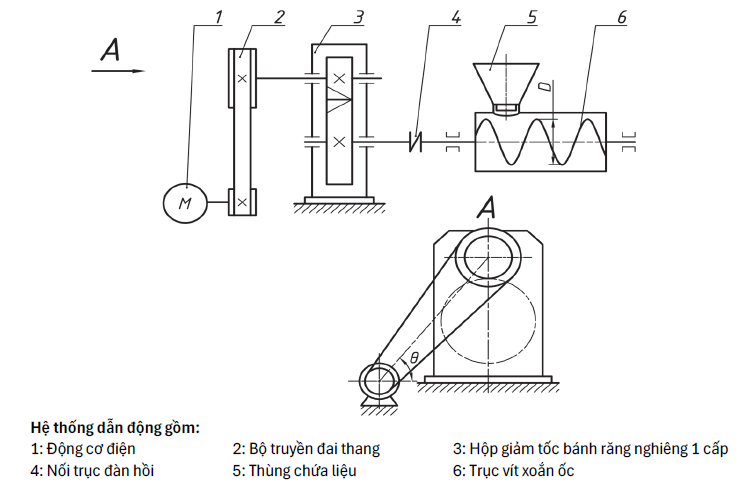
\includegraphics[width=1\textwidth]{pictures/debai.png}
\end{figure}
\begin{center}
\begin{tabular}{|c|c|}
    \hline
    \textbf{Phương án} & \textbf{6} \\
    \hline
    Lực vòng trên cánh vít F, (N) & 2800  \\
    \hline     
    Vận tốc vòng cánh vít v, (m/s) & 1,3  \\
    \hline
    Đường kính cánh vít, D (mm) & 225  \\
    \hline
    Thời gian phục vụ L, (năm) & 7  \\
    \hline
    Số ca làm việc, (ca) & 2  \\
    \hline
    Thời gian làm việc mỗi ca, (giờ) & 8  \\
    \hline
    Số giờ làm việc mỗi năm, (giờ) & 300  \\
    \hline
\end{tabular}
\end{center}
\cleardoublepage
    \chapter{Chọn động cơ điện}
\section{Xác định công suất bộ phận công tác}
\begin{equation}
    P_{ct} = \frac{F.v}{1000} = \frac{2800 \cdot 1.4}{1000} = 3.92 \, \text{kW}
\end{equation}

\section{Số vòng quay của bộ phận công tác}
\begin{equation}
    n_{ct} = \frac{60000.v}{\pi.D} = \frac{60000 \cdot 1.4}{\pi \cdot 225} = 118.84 \, \text{(v/ph)}
\end{equation}

\section{Hiệu suất của các bộ truyền và các cặp ổ trong hệ thống dẫn động}
\begin{itemize}
    \item Bộ truyền đai: $\eta_{d} = 0.96$ 
    \item Bộ truyền bánh răng: $\eta_{br} = 0.98$
    \item Nối trục: $\eta_{nt} = 0.99$
    \item Ổ lăn: $\eta_{ol} = 0.995$
\end{itemize}
Hiệu suất hệ thống:
\begin{equation}
    \eta _{ch} = \eta_{d}\eta_{br}\eta_{nt}(\eta_{ol})^3 = 0.96 \cdot 0.98 \cdot 0.99 \cdot 0.995 = 0.9175
\end{equation}

\section{Công suất động cơ cần thiết}
\begin{equation}
    P_{dc} = \frac{P_{ct}}{\eta_{ch}} = \frac{3.92}{0.9175} = 4.273 \, \text{kW}
\end{equation}

\section{Dãy tỉ số truyền nên dùng cho các bộ truyền trong hệ thống}
\begin{itemize}
    \item Bộ truyền đai thang: $u_{d} = 2...3$
    \item Bộ truyền bánh răng trụ răng nghiêng $u_{br} = 3...5$
\end{itemize}
Như vậy số vòng quay của động cơ dao động trong khoảng từ 713 vòng/phút đến 2971 vòng/phút.\\
Chọn động cơ SGA132S có: $P_{dc} = 5.5 \, \text{kW}$ và $n_{dc} = 1450 \, \text{vòng/phút}$. \\
Như vậy tỉ số truyền chung của hệ thống là:
\begin{equation}
    u_{ch} = \frac{n_{dc}}{n_{ct}} = \frac{1450}{118.82} = 12.202
\end{equation}

\section{Phân phối tỉ số truyền}
Tỷ số truyền của cả hệ được xác định theo công thức:
\begin{equation}
    u_{ch} = u_d.u_{br} = 12.202
\end{equation}
Chọn tỉ số truyền của hộp giảm tốc:
\begin{equation}
    u_{br} = 5
\end{equation}
Như vậy:
\begin{equation}
    u_d = \frac{u_{ch}}{u_{br}} = \frac{12.202}{5} = 2.44
\end{equation}

\section{Tính toán công suất và momen trên các trục}
\subsection{Tính toán công suất trên các trục}
Công suất trên trục công tác:
\begin{equation}
    P_{ct} = \frac{F.v}{1000} = \frac{2800 \cdot 1.4}{1000} = 3.92 \, \text{kW}
\end{equation}
Công suất trên trục II:
\begin{equation}
    P_{II} = \frac{P_{ct}}{\eta_{ol}^2.\eta_{nt}} = \frac{3.92}{0.995^2 \cdot 0.99} = 4 \, \text{kW}
\end{equation}
Công suất trên trục I:
\begin{equation}
    P_{I} = \frac{P_{II}}{\eta_{ol} \cdot \eta_{br}} = \frac{4}{0.995 \cdot 0.98} = 4.102 \, \text{kW}
\end{equation}

\subsection{Tính toán momen trên các trục}
Momen trên trục công tác:
\begin{equation}
    M_{lv} = 9.55 \cdot 10^6 \cdot \frac{P_{ct}}{n_{ct}} = 9.55 \cdot 10^6 \cdot \frac{3.92}{118.82} = 315053.5 \, \text{(N.mm)}
\end{equation}
Momen trên trục II:
\begin{equation}
    M_{II} = 9.55 \cdot 10^6 \cdot \frac{P_{II}}{n_{II}} = 9.55 \cdot 10^6 \cdot \frac{4}{118.82} = 321442.24 \, \text{(N.mm)}
\end{equation}
Momen trên trục I:
\begin{equation}
    M_{I} = 9.55 \cdot 10^6 \cdot \frac{P_{I}}{n_{I}} = 9.55 \cdot 10^6 \cdot \frac{4.102}{594.26} = 65914.97 \, \text{(N.mm)}
\end{equation}
Momen trên trục động cơ:
\begin{equation}
    M_{dc} = 9.55 \cdot 10^6 \cdot \frac{P_{dc}}{n_{dc}} = 9.55 \cdot 10^6 \cdot \frac{4.275}{1450} = 28139.71 \, \text{(N.mm)}
\end{equation}

\section{Bảng thông số hệ thống}
\begin{figure}[H]
    \centering
    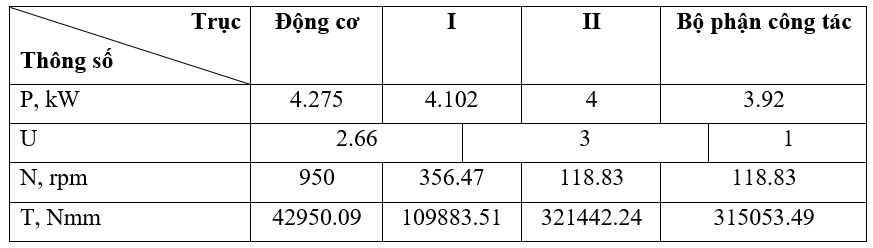
\includegraphics[width=1\textwidth]{pictures/bangdactinh.png}
    \caption{Bảng thông số hệ thống}
\end{figure}
    \chapter{Chọn bộ truyền đai}
\section{Chọn loại đai}
Dựa vào công suất động cơ là $P_{dc} = 4.275 \, \text{kW}$ và số vòng quay $n_{dc} = 1450$ vòng/phút \\
$\Rightarrow$ Chọn đai loại A \\    
\begin{table}[H]
\begin{tabular}{|c|c|c|c|c|c|c|c|}
    \hline 
    Ký hiệu đai & $b_p$  & $b_0$  & h  & $y_0$ (mm) & A ($mm^2$) & Chiều dài đai (m) & $d_{1min} (mm)$ \\ \hline
    A & 11 & 13 & 8 & 2.8 & 81 & 560 $\div$ 4000 & 90 \\ \hline
\end{tabular}
\caption{Thông số đai loại A}
\end{table}
\section{Tính đường kính bánh đai nhỏ}
\begin{equation}
    d_1 = 1.2d_{min} = 1.2 \cdot 90 = 108 \, \text{(mm)}
\end{equation}
Chọn theo dãy giá trị tiêu chuẩn, ta chọn $d_1 = 112 \, \text{(mm)}$.\\
Vận tốc dài trên bánh đai nhỏ:
\begin{equation}
    v_1 = \frac{\pi d_1 n_1}{60000} = \frac{\pi \cdot 112 \cdot 1450}{60000} = 8.503 \, \text{(m/s)}
\end{equation}
$\Rightarrow$ Thỏa điều kiện $v_1 < 25 \, \text{(m/s)}$ \\

\section{Chọn hệ số trượt tương đối và tính đường kính bánh đai lớn}
Chọn hệ số trượt tương đối $\xi = 0.01$. Từ công thức tỉ số của bộ truyền đai:
\begin{equation}
    u_d = \frac{d_2}{d_1 (1 - \xi)}
\end{equation}
\begin{equation}
    d_2 = u_d \cdot d_1 \cdot (1 - \xi) = 2.44 \cdot 112 \cdot (1 - 0.01) = 270.55 \, \text{(mm)}
\end{equation}
Chọn theo dãy giá trị tiêu chuẩn, ta chọn $d_2 = 280 \, \text{(mm)}$.\\
Tính lại tỷ số truyền:
\begin{equation}
    u_d = \frac{d_2}{d_1 (1 - \xi)} = \frac{280}{112 \cdot 0.99} = 2.52
\end{equation}
Để sai số tỷ số truyền bằng 0, ta tính lại đường kính bánh đai nhỏ:
\begin{equation}
    d_1 = \frac{d_2}{u_d \cdot (1 - \xi)} = \frac{280}{2.44 \cdot (1 - 0.01)} = 115.91 \, \text{(mm)}
\end{equation}

\section{Chọn khoảng cách trục $a$}
Theo các thông số $u_d = 2.44$ và $d_2 = 280 \, \text{mm}$:
\begin{equation}
    a = 1.2d_2 = 1.2 \cdot 280 = 336 \, \text{(mm)}
\end{equation}
Chiều dài đai:
\begin{equation}
    L = 2a + \pi \frac{d_1 + d_2}{2} + \frac{(d_2 - d_1)^2}{4a}
\end{equation}
\[
    L = 2 \cdot 336 + \pi \frac{115.91 + 280}{2} + \frac{(280 - 115.91)^2}{4 \cdot 336} = 1313.93 \, \text{(mm)}
\]
$\Rightarrow$ Chọn chiều dài đai $L = 1400 \, \text{mm}$ theo dãy giá trị tiêu chuẩn.\\
Tính lại khoảng cách trục:
\begin{equation}
    k = L - \pi \frac{d_1 + d_2}{2} = 1400 - \pi \frac{115.91 + 280}{2} = 778.106 \, \text{(mm)}
\end{equation}
\begin{equation}
    \Delta = \frac{d_2 - d_1}{2} = \frac{280 - 115.91}{2} = 82.045 \, \text{(mm)}
\end{equation}
\begin{equation}
    a = \frac{k + \sqrt{k^2 - 8\Delta^2}}{4} = \frac{778.106 + \sqrt{778.106^2 - 8 \cdot 82.045^2}}{4} = 380.2 \, \text{(mm)}
\end{equation}
Kiểm tra $a$ thỏa điều kiện:
\begin{equation}
    2(d_1 + d_2) \geq a \geq 0.7(d_1 + d_2)
\end{equation}
\[
    2(115.91 + 280) \geq a \geq 0.7(115.91 + 280)
\]
\[
    791.82 \geq a \geq 277.173
\]
$\Rightarrow a = 380.2 \, \text{(mm)}$ thỏa điều kiện. \\

\section{Tính toán vận tốc đai và số truyền đai}
Vận tốc dây đai:
\begin{equation}
    v = \frac{\pi d_1 n_1}{60000} = \frac{\pi \cdot 115.91 \cdot 1450}{60000} = 8.8 \, \text{(m/s)}
\end{equation}
Số vòng chạy đai trong 1 giây:
\begin{equation}
    i = \frac{v_1}{L} = \frac{8.8}{1400 \cdot 10^{-3}} = 6.286 \, \text{s}^{-1}
\end{equation}
$\Rightarrow$ Thỏa điều kiện $i \leq [i] = 10 \, \text{s}^{-1}$. \\

\section{Tính góc ôm đai bánh nhỏ}
\begin{equation}
    \alpha_1 = 180 - 57 \frac{d_2 - d_1}{a} = 180 - 57 \frac{280 - 115.91}{380.2} = 155.29^{\circ}
\end{equation}
\section{Các hệ số sử dụng}
Hệ số xét đến ảnh hưởng góc ôm đai:
\begin{equation}
    C_{\alpha} = 1.24(1 - e^{\frac{-\alpha_1}{110}}) = 1.24(1 - e^{\frac{-155.29}{110}}) = 0.938
\end{equation}

Hệ số xét đến ảnh hưởng vận tốc:
\begin{equation}
    C_v = 1 - 0.05(0.01v^2 - 1) = 1 - 0.05(0.01 \cdot 8.8^2 - 1) = 1.011
\end{equation}

Hệ số xét đến ảnh hưởng tỷ số truyền $u$:
\begin{equation}
    C_u = 1.14 \quad (v > 2.5 \, \text{m/s})
\end{equation}

Hệ số xét đến ảnh hưởng của chiều dài đai $L$:
\begin{equation}
    C_L = \sqrt[6]{\frac{L}{L_0}} = \sqrt[6]{\frac{1400}{1700}} = 0.968
\end{equation}

Hệ số xét đến sự ảnh hưởng của sự phân bố không đều tải trọng giữa các dây đai:
\begin{equation}
    C_z = 0.95 \quad \text{(chọn sơ bộ)}
\end{equation}

Hệ số xét đến ảnh hưởng của chế độ tải trọng:
\begin{equation}
    C_r = 0.9 \quad \text{(chọn sơ bộ)}
\end{equation}

Chọn công suất có ích cho phép theo GOST 1284.3 - 96, ta có: \\
Đai loại A, $d_1 = 115.91 \, \text{mm}$, $v_1 = 8.8 \, \text{m/s}$ \\
$\Rightarrow$ Chọn $[P_0] = 1.80$.

Tính số dây đai theo công thức:
\begin{equation}
    z \geq \frac{P_1}{[P_0] \cdot C_{\alpha} \cdot C_u \cdot C_L \cdot C_z \cdot C_r \cdot C_v} = \frac{4.102}{1.8 \cdot 0.938 \cdot 1.14 \cdot 0.968 \cdot 0.95 \cdot 0.9 \cdot 1.011} = 2.55
\end{equation}
$\Rightarrow$ Chọn $z = 3$ dây đai. \\
Kiểm nghiệm lại $C_z$: vì $z = 3$ nên $C_z = 0.95$ như đã chọn sơ bộ.

\section{Lực trên dây đai}
Tổng lực căng đai ban đầu trên cả dây đai:
\begin{equation}
    F_0 = z \cdot A \cdot [\sigma_0] = 3 \cdot 81 \cdot 1 = 243 \, \text{(N)}
\end{equation}
Trong đó: Đối với đai thang, $\sigma_0 \leq 1.5 \, \text{MPa}$ nên ta chọn $\sigma_0 = 1 \, \text{MPa}$, $z = 3$, $A = 81 \, \text{mm}^2$.

Lực căng trên mỗi dây đai:
\begin{equation}
    \frac{F_0}{z} = \frac{243}{3} = 81 \, \text{(N)}
\end{equation}

Tổng lực vòng có ích trên cả 3 đai:
\begin{equation}
    F_t = \frac{1000P_1}{v_1} = \frac{1000 \cdot 4.102}{8.8} = 466.136 \, \text{(N)}
\end{equation}

Lực vòng có ích trên mỗi dây đai:
\begin{equation}
    \frac{F_t}{z} = \frac{466.136}{3} = 155.379 \, \text{(N)}
\end{equation}

\section{Lực tác dụng lên trục}
\begin{equation}
    F_r \approx 2F_0\sin\left(\frac{\alpha_1}{2}\right) = 2 \cdot 243 \sin\left(\frac{155.29}{2}\right) = 474.744 \, \text{(N)}
\end{equation}

\section{Ứng suất lớn nhất trong dây đai}
\begin{equation}
    \sigma_{max} = \sigma_1 + \sigma_v + \sigma_{F1} = \sigma_0 + 0.5\sigma_t + \sigma_v + \sigma_{F1}
\end{equation}
\begin{equation}
    = \frac{F_0}{A} + 0.5 \cdot \frac{F_t}{A} + \rho \cdot v^2 \cdot 10^{-6} + E \cdot \frac{2 \cdot y_0}{d_1}
\end{equation}
\[
    = \frac{243}{3 \cdot 81} + 0.5 \cdot \frac{466.136}{3 \cdot 81} + 1000 \cdot 8.8^2 \cdot 10^{-6} + 60 \cdot \frac{2 \cdot 2.8}{115.19} = 4.88 \, \text{(MPa)}
\]

\section{Tuổi thọ dây đai}
\begin{equation}
    L_h = \frac{\left(\frac{\sigma_r}{\sigma_{max}}\right)^m \cdot 10^7}{2 \cdot 3600 \cdot i} = \frac{\left(\frac{9}{6.9}\right)^8 \cdot 10^7}{2 \cdot 3600 \cdot 6.286} = 29571.59 \, \text{(h)}
\end{equation}
Trong đó:
\begin{itemize}
    \item $\sigma_r = 9 \, \text{(MPa)}$ - giới hạn mỏi của đai thang.
    \item $m = 8$ - chỉ số mũ của đường cong mỏi đối với đai thang.
    \item $i = 6.286 \, \text{(s}^{-1}\text{)}$ - số vòng chạy của đai trong một giây.
\end{itemize}
\section{Bảng thông số bộ truyền đai}
\begin{table}[H]
    \centering
    \begin{tabular}{|l|c|}
        \hline
        \textbf{Thông số} & \textbf{Giá trị} \\ \hline
        Loại đai & A \\ \hline
        Đường kính bánh dẫn, $d_1$ (mm) & 115.91 \\ \hline
        Đường kính bánh bị dẫn, $d_2$ (mm) & 280 \\ \hline
        Chiều dài dây đai, $L$ (mm) & 1400 \\ \hline
        Khoảng cách trục, $a$ (mm) & 380.2 \\ \hline
        Góc ôm đai, $\alpha_1$ ($^\circ$) & 155.29 \\ \hline
        Số dây đai, $z$ & 3 \\ \hline
        Tuổi thọ đai, $L_h$ (h) & 29571.59 \\ \hline
    \end{tabular}
    \caption{Bảng thông số bộ truyền đai}
\end{table}
\cleardoublepage
    \section{Tính toán hộp giảm tốc bánh răng nghiêng 1 cấp}
\subsection{Chọn vật liệu cho bánh dẫn và bánh bị dẫn}
Hộp giảm tốc chịu công suất không quá lớn nên chỉ cần chọn vật liệu có độ cứng HB $\leq$ 350.
\begin{itemize}
    \item Bánh dẫn: thép c45 tôi cải thiện 	Bánh dẫn: thép c45 tôi cải thiện đạt độ rắn HB 230…280 có $\sigma_{b1} = 850MPa; \sigma_{ch1} = 650MPa; HB_1 = 250$
    \item o	Bánh bị dẫn: thép c45 tôi cải thiện đạt độ rắn HB 192…240 có $\sigma_{b2} = 750MPa; \sigma_{ch2} = 450MPa; HB_2 = 235$
\end{itemize}
\subsection{Số chu kỳ làm việc cơ sở}
\begin{center}
        $N_{HO_1} = 30.HB_1^{2,4} = 30.250^{2,4} = 1,71.10^7$ chu kỳ \\
        $N_{HO_2} = 30.HB_2^{2,4} = 30.235^{2,4} = 1,47.10^7$ chu kỳ \\
        $N_{FO_1} = N_{FO_2} = 5.10^6$ chu kỳ \\
\end{center}
\subsection{Số chu kỳ làm việc tương đương, xác định theo sơ đồ tải trọng}
\begin{center}
    $N_{HE_1} = 60.c.n.L_h = 60.1.482,5.14400 = 41,69.10{-7}$ chu kỳ
\end{center}
Với c = 1; n = 482,5 vòng/phút; $L_h$= 6.300.8 = 14400 giờ. 
\begin{center}
    $N_{HE_2} = \frac{N_{HE_1}}{\mu} = \frac{41,69.10^7}{6,3} = 6,617.10^7$ chu kỳ
\end{center}
Tương tự:
\begin{center}
    $N_{FE_1} = 60.c.n.L_h = 60.1.76,6.14400 = 6,618.10^{-7}$ chu kỳ
\end{center}
\begin{center}
    $N_{FE_2} = \frac{N_{FE_1}}{\mu} = \frac{41,69.10^7}{6,3} = 6,617.10^7$ chu kỳ
\end{center} 
Vì $N_{HE_1} > N_{HO_1}; N_{HE_2} > N_{HO_2}; N_{FE_1} > N_{FO_1}; N_{FE_2} > N_{FO_2}$ \\
$\Rightarrow K_{HL_1} = K_{HL_2} = K_{FL_1} = K_{FL_2} = 1$
\subsection{Giới hạn mỏi tiếp xúc và giới hạn mỏi uốn}
\[
    \sigma_{OH_{lim}} = 2HB + 70 
\]
\[
    \Rightarrow \sigma_{OH_{lim1}} = 2.250 + 70 = 570MPa
\]
\[
    \Rightarrow \sigma_{OH_{lim2}} = 2.235 + 70 = 540MPa
\]
\[
    \sigma_{OF_{lim}} = 1.8HB
\]
\[
    \Rightarrow \sigma_{OF_{lim1}} = 1.8.250 = 450MPa
\]
\[
    \Rightarrow \sigma_{OF_{lim2}} = 1.8.235 = 423MPa
\]
\subsection{Ứng suất tiếp xúc cho phép}
\[
    [\sigma_{H}] = \frac{\sigma_{OH_{lim}}.Z_R.Z_V.Z_L.Z_XH}{s_H}.K_{HL} = \frac{\sigma_{OH_{lim}}.0,9}{s_H}.K_{HL}
\]
Khi tôi cải thiện $s_H = 1,1$, do đó:
\[
    [\sigma_{H_1}] = \frac{570.0,9}{1,1}.1 = 466,37MPa
\]
\[
    [\sigma_{H_2}] = \frac{540.0,9}{1,1}.1 = 441,82MPa
\]
Ứng suất tính toán cho phép:
\[
    [\sigma_H] = 0,45.([\sigma_{H1}] + [\sigma_{H2}]) = 0,45.(466,37 + 441,82) = 408,68MPa
\]
Tuy nhiên
\[
    [\sigma_{min}] \leq [\sigma_H] \leq 1,25[\sigma_{min}] \Leftrightarrow 441.82 \leq [\sigma_H] \leq 552,275
\]
$\Rightarrow$ Ta chọn $[\sigma_H] = [\sigma_{H2}] = 441,82$ MPa
\subsection{Ứng suất uốn cho phép}
\[
    [\sigma_F] =\frac{\sigma_{OFlim}}{s_F}.K_{HL}
\]
Chọn $s_F = 1,75$, ta có: \\
\[
    [\sigma_{F1}] =\frac{\sigma_{OF1lim}}{s_F}.K_{HL} = \frac{450}{1,75}.1 = 257,143 (MPa)
\]
\[
    [\sigma_{F2}] =\frac{\sigma_{OF2lim}}{s_F}.K_{HL} = \frac{423}{1,75}.1 = 241,7 (MPa)
\]
\subsection{Khoảng cách trục}
Do bánh răng nằm đối xứng các ổ trục nên $\Psi_{ba} = 0,3 \div 0,5$, chọn $\Psi_{ba} = 0,4$ \\
Khi đó $\Psi_{bd} = \frac{\Psi_{ba}.(u+1)}{2} = \frac{0,4.(6,3+1)}{2} = 1,46$ \\
Từ đó tra theo bảng 6.4 ta chọn: $K_{H\beta} = 1,07$, $K_{F\beta} = 1,14$ \\
Tính khoảng cách trục: \\
\[
    a_w = 500.(u+1).\sqrt[3]{\frac{T_1.K_{H\beta}}{\Psi_{ba}.[\sigma_H]^2.u}} = 500.(6,3+1).\sqrt[3]{\frac{63,73.1,07}{0,4.408,68^2.6,3}} = 198,98 (mm)
\]
Theo tiêu chuẩn ta chọn $a_w = 200mm$
\subsection{Môđun răng}
\[
    m_n = (0,01 \div 0,02).a_w = 2 \div 4
\]
Theo tiêu chuẩn ta chọn $m_n = 4$
\subsection{Số răng}
Từ điều kiện $20^\circ \leq \beta \leq 8^\circ$ \\
\[
    \Leftrightarrow \frac{2.a_w.\cos8^\circ}{m_n.(u+1)} \leq z_1 \leq \frac{2.a_w.\cos20^\circ}{m_n.(u+1)}
\]
\[
    \Leftrightarrow \frac{2.200.\cos8^\circ}{4.(6,3+1)} \leq z_1 \leq \frac{2.200.\cos20^\circ}{4.(6,3+1)}
\]
\[
    \Leftrightarrow 13,56 \leq z_1 \leq 12,87
\]
$\Rightarrow$ Chọn $z_1 = 13 \Rightarrow z_2 = u.z_1 = 6,3.13 = 81,9$ \\
$\Rightarrow$ Chọn $z_2 = 82$ \\
Góc nghiêng răng: 
\[
    \beta = \arccos\frac{m_n.(z_1+z_2)}{2.a_w} = \arccos\frac{4.(13+82)}{2.200} = 18,2^\circ
\]
\subsection{Tỉ số truyền sau khi chọn răng}
\[
    u = \frac{z_2}{z_1} = \frac{82}{13} = 6,308
\]
\subsection{Các thông số hình học}
Đường kính vòng chia: \\
\[
    d_1 = \frac{m_n.z_1}{\cos\beta} = \frac{4.13}{\cos18,2^\circ} = 54,738 (mm)
\]
\[
    d_2 = \frac{m_n.z_2}{\cos\beta} = \frac{4.82}{\cos18,2^\circ} = 345,27 (mm)
\]
Đường kính vòng đỉnh: \\
\[
    d_{a1} = d_1 + 2.m_n = 54,738 + 2.4 = 62,738 (mm)
\]
\[
    d_{a2} = d_2 + 2.m_n = 354,27 + 2.4 = 362,27 (mm)
\]
Đường kính vòng đáy: \\ 
\[
    d_{f1} = d_1 - 2,5m_n = 62,738 - 2,5.4 = 44,738 (mm)
\]
\[
    d_{f2} = d_2 - 2,5m_n = 345,27 - 2,5.4 = 335,27 (mm)
\]
Tính lại khoảng cách trục: \\
\[
    a_w = \frac{m_n.(z_1+z_2)}{2\cos\beta} = \frac{4.(13+82)}{2.\cos18,2^\circ} = 200(mm)
\]
Chiều rộng vành răng: 
\begin{itemize}
    \item Bánh bị dẫn: $b_2 = \Psi_{ba}.a_w = 0,4.200 = 80(mm)$
    \item Bánh dẫn: $b_1 = b_2 + 5 = 85(mm)$
\end{itemize}
\subsection{Vận tốc vòng bánh răng}
\[
    v = \frac{\pi.d_1.n_1}{60000} = \frac{\pi.54,738.482,5}{60000} = 1,38 (m/s)
\]
Theo bảng 6.3 ta chọn cấp chính xác 9 với $v_{gh} = 6 m/s$
\subsection{Tính toán kiểm nghiệm giá trị ứng suất tiếp xúc}
Theo bảng 6.6 ta chọn hệ số tải trọng động $K_{HV} = 1,11$, $K_{FV} = 1,22$ \\
\[
    \sigma_H = \frac{z_M.z_H.z_\epsilon}{d_1}.\sqrt{\frac{2.T_1.10^3.K_{H\beta}.K_{HV}.(u+1)}{b_w.u}} 
\]
\[
    = \frac{190.2,3847.0,8124}{54,738}.\sqrt{\frac{2.63,73.10^3.1,07.1,11.(6,3+1)}{80.6,3}} = 314,887 (MPa)
\]
Với:
\begin{itemize}
    \item $Z_M = 190$ vì vật liệu bằng thép
    \item $Z_H = \sqrt{\frac{4.\cos\beta}{\sin(2.\alpha_{tw})}} = \sqrt{\frac{4.\cos18,2}{\sin(2.20,9637)}} = 2,3847$
    \item $\alpha_{tw} = \arctan(\frac{\tan\alpha_{nw}}{\cos\beta}) = \arctan(\frac{\tan20}{\cos18,2}) = 20,9637$
    \item $Z_\epsilon = \sqrt{\frac{1}{\epsilon_\alpha}} = \sqrt{\frac{1}{1,515}} = 0,8124$
    \item $\epsilon_\alpha = [1,88-3,2.(\frac{1}{z_1}+\frac{1}{z_2})].\cos\beta = [1,88-3,2.(\frac{1}{13}+\frac{1}{82})].\cos18,2 = 1,515$
\end{itemize}
\[
    \sigma_H = 314,887 MPa \leq 441,82 MPa
\]
    $\Rightarrow \sigma_H \leq [\sigma_H]$ thỏa mãn\\
\subsection{Số răng tương đương}
\[
    z_{v1} = \frac{z_1}{\cos^3(\beta)} = \frac{13}{\cos^3(18,2)} = 13,685 \Rightarrow z_{v1} = 14
\]
\[
    z_{v2} = \frac{z_2}{\cos^3(\beta)} = \frac{82}{\cos^3(18,2)} = 86,32 \Rightarrow z_{v1} = 87
\]
\subsection{Hệ số dạng răng}
\begin{itemize}
    \item Đối với bánh dẫn: $Y_{F1} = 3,47 + \frac{13,2}{z_{v1}} = 3,47 + \frac{13,2}{14} = 4,413$
    \item Đối với bánh bị dẫn: $Y_{F2} = 3,47 + \frac{13,2}{z_{v2}} = 3,47 + \frac{13,2}{87} = 3,622$
\end{itemize}
\subsection{Ứng suất uốn tính toán}
Đặc tính so sánh độ bền uốn:
\begin{itemize}
    \item Bánh dẫn: $\frac{[\sigma_{F1}]}{Y_{F1}} = \frac{257,143}{4,413} = 58,27$
    \item Bánh bị dẫn: $\frac{[\sigma_{F2}]}{Y_{F2}} = \frac{241,7}{3,622} = 66,73$
\end{itemize}
$\Rightarrow$ Ta kiểm tra độ bền uốn theo bánh dẫn có độ bền thấp hơn:\\
Ứng suất uốn tính toán:
\[
    \sigma_{F1} = \frac{Y_{F1}.F_t.K_{F1}.Y_\epsilon.Y_\beta}{b_2.m} = \frac{4,413.2328,547.1,39.0,66.0,6985}{80.4} = 20,577 (MPa)
\] 
Với: 
\begin{itemize}
    \item $Y_\epsilon = \frac{1}{\epsilon_\alpha} = \frac{1}{1,515} = 0,66$
    \item $F_t = 2.10^3.\frac{T_1}{d_{w1}} = 2.10^3.\frac{63,73}{54,738} = 2328,547$
    \item $Y_\beta = 1 - \epsilon_\beta\frac{\beta}{120} = 1 - 1,988\frac{18,2}{120} = 0,6985$
    \item $\epsilon_\beta = b_w.\frac{\sin\beta}{\pi.m} = 80.\frac{\sin18,2}{\pi.4} = 1,988$
    \item $K_{F1} = K_{F\alpha}.K_{F\beta}.K_{FV} = 1.1,14.1,22 = 1,39$
    \item $K_{F\alpha} = \frac{4 + (\epsilon_\alpha - 1).(n_{cx} - 5)}{4\epsilon_\alpha} = \frac{4 + (1,515 - 1).(9 - 5)}{4.1,515} = 1$
\end{itemize}
$\Rightarrow \sigma_{F1} < [\sigma_{F1}] = 257,143$ MPa do đó độ bền uốn thỏa\\
\subsection{Phân tích lực}
\begin{figure}[H]
    \centering
    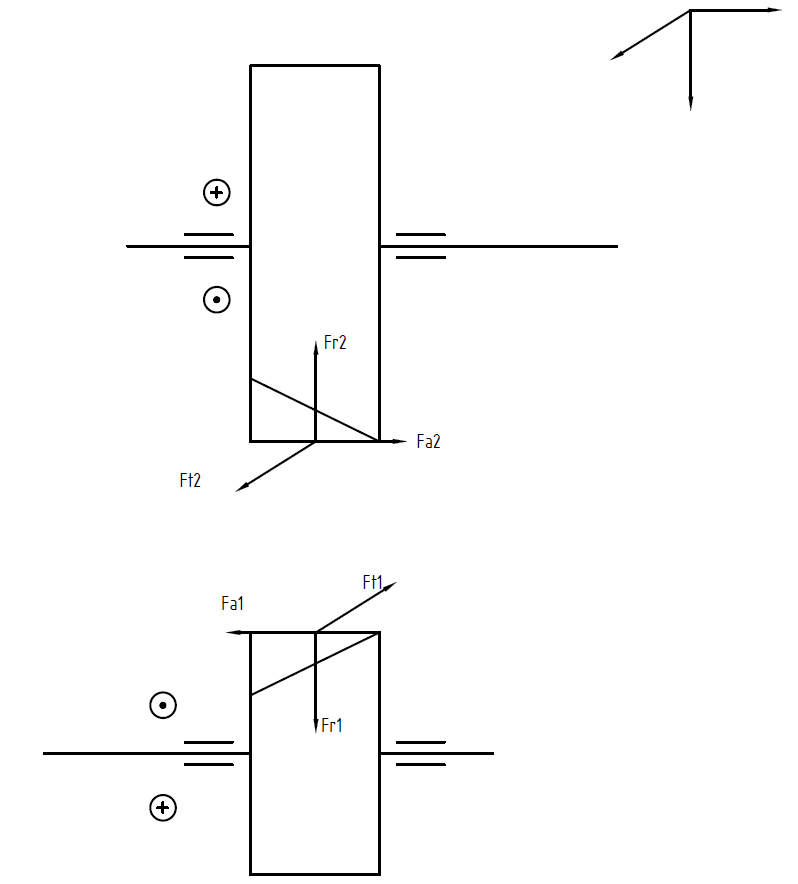
\includegraphics[width=0.5\textwidth]{pictures/phantichluc.png}
\end{figure}
\cleardoublepage
    \chapter{Tính toán trục}
\section{Chọn vật liệu và tính sơ bộ}
Vì chưa biết chiều dài trục nên ta thiết kế sơ bộ để xác định đường kính trục theo moment xoắn. 
Chọn vật liệu chế tạo trục là thép C45 tôi cải thiện. Do trục bánh răng trong hộp giảm tốc là chi tiết máy rất quan trọng.

Tra bảng thông số vật liệu ta có thông số cơ tính của vật liệu như sau:
\begin{itemize}
    \item Loại thép: 45
    \item Nhiệt luyện: tôi cải thiện
    \item Độ rắn: $HB_1 = 260 \, \text{HB}$
    \item Giới hạn bền: $\sigma_b = 850 \, \text{MPa}$
    \item Giới hạn chảy: $\sigma_{ch} = 650 \, \text{MPa}$
\end{itemize}
Chọn ứng suất xoắn cho phép $[\tau] = 20 \, \text{MPa}$ \\
Xác định sơ bộ đường kính trục:
\begin{equation}
d_1 \geq \sqrt[3]{\frac{T_1}{0.2[\tau]}} = \sqrt[3]{\frac{65914.47}{0.2 \cdot 20}} = 25.44 \text{mm}
\end{equation}
\begin{equation}
d_2 \geq \sqrt[3]{\frac{T_2}{0.2[\tau]}} = \sqrt[3]{\frac{321365.99}{0.2 \cdot 20}} = 37.69 \text{mm}
\end{equation}
Tra bảng 10.2 tài liệu [2], ta chọn sơ bộ đường kính trục và bề rộng ổ lăn theo tiêu chuẩn:
\begin{itemize}
    \item Trục I: $d_1 = 25.44 \, \text{mm}$; $b_{o1} = 19 \, \text{mm}$
    \item Trục II: $d_2 = 35 \, \text{mm}$; $b_{o2} = 25 \, \text{mm}$  
\end{itemize}
\section{Xác định khoảng cách giữa các ổ lăn và điểm đặt lực}
\subsection{Trục I}
Theo bảng 10.3 tài liệu [2], ta có:
\begin{itemize}
    \item $k_1 = 8$ mm: Khoảng cách từ mặt mút của chi tiết quay đến thành trong của hộp hoặc khoảng cách giữa các chi tiết quay
    \item $k_2 = 10$ mm: Khoảng cách từ mặt mút ổ đến thành trong của hộp
    \item $k_3 = 10$ mm: Khoảng cách từ mặt mút của chi tiết quay đến nắp ổ
    \item $h_n = 15$ mm: Chiều cao nắp ổ và đầu bu lông
    \item Chọn sơ bộ chiều dài mayơ bánh răng trụ dẫn: $l_{m13}$ = bề dày bánh răng $b_w$ = 70 mm
    \item Chọn sơ bộ chiều dài mayơ bánh đai: $l_{m12} = (1.2\div 1.5)d_1 = 30 \div 37.5$. Chọn $l_{m22}=36$ mm 
    \item $l_{13} = 0.5(l_{m13} + b_{o1}) + k_1 + k_2 = 0.5(70 + 21) + 10 + 8 = 63.5 \, \text{mm}$
    \item $l_{11} = 2l_{13} = 2 \cdot 63.5 = 127 \, \text{mm}$
 
    \item $l_{12} = 0.5(l_{m12} + b_{o1}) + k_3 + h_n = 0.5(50 + 21) + 10 + 15 = 75.5 \, \text{mm}$
\end{itemize}

\subsection{Trục II}
Theo bảng 10.3 tài liệu [2], ta có:
\begin{itemize}
    \item $k_1 = 8$ mm: Khoảng cách từ mặt mút của chi tiết quay đến thành trong của hộp hoặc khoảng cách giữa các chi tiết quay
    \item $k_2 = 10$ mm: Khoảng cách từ mặt mút ổ đến thành trong của hộp
    \item $k_3 = 10$ mm: Khoảng cách từ mặt mút của chi tiết quay đến nắp ổ
    \item $h_n = 15$ mm: Chiều cao nắp ổ và đầu bu lông
    \item $l_{m23}$ = bề dày bánh răng $b_w$ = 64 mm
    \item $l_{m22} = (1.2\div 1.5)d_1 = 45.25 \div 57$. Chọn $l_{m22}=57$ mm
    \item $l_{23} = 0.5(l_{m13} + b_{o1}) + k_1 + k_2 = 64.5 \, \text{mm}$
    \item $l_{21} = 0.5(l_{m23} + b_{o2}) + k_1 + k_2 = 140.5 \, \text{mm}$
    \item $l_{22} = 2l_{21}$ = 281 mm
\end{itemize}

\section{Phân tích lực tác dụng}
\subsection{Trục I}
\begin{itemize}
    \item Lực vòng: $F_{t1}$ = 2471.8 N
    \item Lực dọc trục: $F_{a1}$ = 756.18 N
    \item Lực hướng tâm: $F_{r1}$ = 940.82 N 
    \item Lực do bộ truyền đai: $F_d$ = 474.74 N
\end{itemize}
\subsection{Trục II}
\begin{itemize}
    \item Lực vòng: $F_{t2}$ = 2471.8 N
    \item Lực dọc trục: $F_{a2}$ = 940.82 N
    \item Lực hướng tâm: $F_{r2}$ = 756.18 N 
    \item Lực nối trục: $F_{nt}$ = 1483.23 N
\end{itemize}
\section{Tính momen tương đương và đường kính trục}
\subsection{Trục I}
Moment do lực dọc trục tạo ra:
\begin{equation}
    M_{a1} = F_{a1} \cdot \frac{d_1}{2} 
           = 756.177 \cdot \frac{53.33}{2} 
           = 20163.47\ \text{Nmm}
\end{equation}
\[
    \left\{
    \begin{array}{l}
        \sum F_X = 0 \\
        \sum F_Y = 0 \\
        \sum M_{Y/A} = 0 \\
        \sum M_{X/A} = 0
    \end{array}
    \right.
    \Leftrightarrow
    \left\{
    \begin{array}{l}
        -F_{dx} - R_{BX} + F_{t1} - R_{DX} = 0 \\
        -F_{dy} - R_{BY} + F_{r1} - R_{DY} = 0  \\
        -52 R_{BX} + 116.5 F_{t1} - 181R_{DX} = 0 \\
        -52 R_{BY} + 116.5 F_{r1} - M_{a1} - 181 R_{DY} = 0
    \end{array}
    \right.
    \Leftrightarrow
    \left\{
    \begin{array}{l}
        R_{BX} = 1879.31\ \text{N} \\
        R_{BY} = 454.31\ \text{N} \\
        R_{DX} = 1051.05\ \text{N} \\
        R_{DY} = 363.63\ \text{N}
    \end{array}
    \right.
\]
\begin{figure}[H]
    \centering
    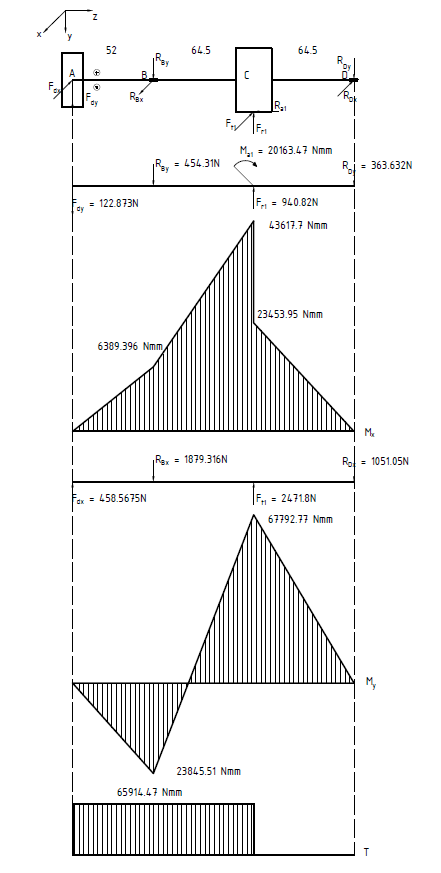
\includegraphics[width=0.75\textwidth]{pictures/momen1.png}
    \caption{Biểu đồ momen trên trục I}    
\end{figure}
\begin{equation}
    M_A^{td} 
    = \sqrt{M_{X/A}^2 + M_{Y/A}^2 + 0.75 \cdot T_A^2} 
    = \sqrt{0.75 \cdot 65914.47^2}  
    = 57083.6\ \text{Nmm}
\end{equation}

\[
    M_B^{td} 
    = \sqrt{M_{X/B}^2 + M_{Y/B}^2 + 0.75 \cdot T_B^2} 
    = \sqrt{6389.396^2 + 23845.51^2 + 0.75 \cdot 65914.47^2} 
    = 62193.01\ \text{Nmm}
\]

\[
    M_C^{td} 
    = \sqrt{M_{X/C}^2 + M_{Y/C}^2 + 0.75 \cdot T_C^2} 
    = \sqrt{43617.7^2 + 67792.77^2 + 0.75 \cdot 65914.47^2} 
    = 98777.03\ \text{Nmm}
\]

\begin{equation}
    M_D^{td} 
    = \sqrt{M_{X/D}^2 + M_{Y/D}^2 + 0.75 \cdot T_D^2} 
    = 0 
\end{equation}
$\Rightarrow$ Vị trí nguy hiểm là vị trí C.
\begin{equation}
    d_C \ge \sqrt[3]{\frac{M_C^{td}}{0.1 \cdot \sigma}} 
        = \sqrt[3]{\frac{98777.03}{0.1 \cdot 67}} 
        = 24.5\ \text{mm}
\end{equation}
Tại ví trí C có lắp bánh răng, do đó ta tăng đường kính trục thêm 5\% = 25.7 mm. \\
Căn cứ theo kết cấu của trục và bánh răng dẫn, thiết kế trục dẫn 1 với bánh răng liền trục, đường kính các tiết diện còn lại chọn để thỏa mãn yêu cầu về lắp ráp và thỏa mãn dãy kích thước tiêu chuẩn: 
\begin{itemize}
    \item $d_A$ = 22 mm
    \item $d_B$ = 30 mm
    \item $d_D$ = 30 mm
\end{itemize}

\subsection{Trục II}
Moment do lực dọc trục tạo ra:
\begin{equation}
    M_{a2} = F_{a2} \cdot \frac{d_2}{2} 
           = 756.177 \cdot \frac{266.67}{2} 
           = 100825\ \text{Nmm}
\end{equation}
\[
    \left\{
    \begin{array}{l}
        \sum F_X = 0 \\
        \sum F_Y = 0 \\
        \sum M_{Y/A} = 0 \\
        \sum M_{X/A} = 0
    \end{array}
    \right.
    \Leftrightarrow
    \left\{
    \begin{array}{l}
        R_{AX} - F_{t2} - R_{CX} + F_{nt} = 0 \\
        -R_{AY} - F_{r2} + R_{CY} \\
        -76 F_{t2} - 140.5 R_{CX} + 205 F_{nt} = 0 \\
        -76 F_{r2} + 140.5 R_{CY} - M_{a1} = 0
    \end{array}
    \right.
    \Leftrightarrow
    \left\{
    \begin{array}{l}
        R_{AX} = 1815.8\ \text{N} \\
        R_{AY} = 287.235\ \text{N} \\
        R_{CX} = 827.235\ \text{N} \\
        R_{CY} = 1228.49\ \text{N}
    \end{array}
    \right.
\]
\begin{figure}[H]
    \centering
    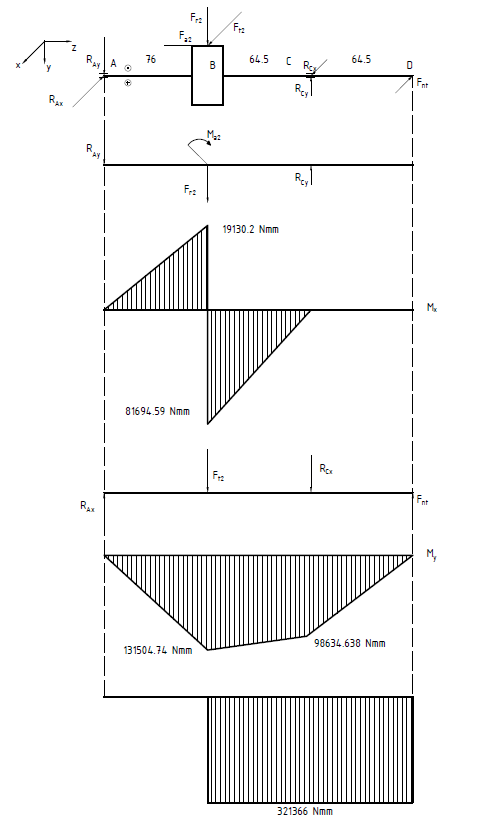
\includegraphics[width=0.85\textwidth]{pictures/momen2.png}
    \caption{Biểu đồ momen trên trục II}
\end{figure}
\begin{equation}
    M_A^{td} 
    = \sqrt{M_{X/A}^2 + M_{Y/A}^2 + 0.75 \cdot T_A^2} 
    = 0
\end{equation}

\[
    M_B^{td} 
    = \sqrt{M_{X/B}^2 + M_{Y/B}^2 + 0.75 \cdot T_B^2} 
    = \sqrt{81694.59^2 + 131504.74^2 + 0.75 \cdot 321366^2} 
    = 318472.26\ \text{Nmm}
\]

\[
    M_C^{td} 
    = \sqrt{M_{X/C}^2 + M_{Y/C}^2 + 0.75 \cdot T_C^2} 
    = \sqrt{98634.638^2 + 0.75 \cdot 321366^2} 
    = 295272.54\ \text{Nmm}
\]

\[
    M_D^{td} 
    = \sqrt{M_{X/D}^2 + M_{Y/D}^2 + 0.75 \cdot T_D^2} 
    = \sqrt{0.75 \cdot 321366^2} 
    = 278311.12\ \text{Nmm}
\]
$\Rightarrow$ Vị trí nguy hiểm là vị trí B.
\begin{equation}
    d_B \ge \sqrt[3]{\frac{M_B^{td}}{0.1 \cdot \sigma}} 
        = \sqrt[3]{\frac{318472.26}{0.1 \cdot 67}} 
        = 36.22\ \text{mm}
\end{equation}
Tại ví trí B có lắp bánh răng, do đó ta tăng đường kính trục thêm 5\% = 38 mm. \\
Như vậy, để thỏa mãn dãy kích thước tiêu chuẩn và yêu cầu lắp ráp, ta chọn:
\begin{itemize}
    \item $d_A$ = 40 mm
    \item $d_B$ = 45 mm     
    \item $d_C$ = 40 mm
    \item $d_D$ = 36 mm
\end{itemize}

\section{Tính toán và kiểm nghiệm then}
\subsection{Xác định ứng suất dập cho phép và ứng suất cắt cho phép của then tại các vị trí lắp ráp}
\subsubsection{Mối ghép then tại tiết diện lắp bánh đai trên trục I}
\begin{itemize}
    \item Do bánh đai được chế tạo từ gang ở chế độ tải trọng tĩnh, ta có ứng suất dập cho phép của then $[\sigma_d] = 80 \, MPa$ (Bảng 9.5, [2]).
    \item Ứng suất cắt cho phép của then $[\tau_c] = 60 \dots 90 \, MPa$, ta chọn $[\tau_c] = 60 \, MPa$.
    \item Dựa vào đường kính trục và bảng 9.1a [2], ta chọn then bằng cho mối ghép trên và có kích thước sau:
    \begin{table}[h!]
    \centering
    \begin{tabular}{|c|c|c|c|c|}
    \hline
    $\mathbf{d}$ & $\mathbf{b}$ & $\mathbf{h}$ & $\mathbf{t_1}$ & $\mathbf{t_2}$ \\
    \hline
    22 & 8 & 7 & 4 & 2.8 \\
    \hline
    \end{tabular}
    \caption{Kích thước then tại vị trí lắp bánh đai trên trục I}
    \end{table}
\end{itemize}
\subsubsection{Các mối ghép then trên trục II}
\begin{itemize}
    \item Do bánh răng và nối trục đều được chế tạo từ thép nên ở chế độ tải trọng tĩnh, ta có ứng suất dập cho phép của then $[\sigma_d] = 150 \, MPa$ (Bảng 9.5, Trịnh Chất tập 1).
    \item Ứng suất cắt cho phép của then $[\tau_c] = 60 \dots 90 \, MPa$, ta chọn $[\tau_c] = 60 \, MPa$.
    \item Dựa vào đường kính trục và bảng 9.1a (Trịnh Chất, tập 1), ta chọn then bằng cho mối ghép trên và có kích thước sau:
    \begin{itemize}
        \item Tại vị trí lắp bánh răng:
        \begin{table}[h!]
        \centering
        \begin{tabular}{|c|c|c|c|c|}
        \hline
        $\mathbf{d}$ & $\mathbf{b}$ & $\mathbf{h}$ & $\mathbf{t_1}$ & $\mathbf{t_2}$ \\
        \hline
        45 & 14 & 9 & 5.5 & 3.8 \\
        \hline
        \end{tabular}
        \caption{Kích thước then tại vị trí lắp bánh răng trên trục II}
        \end{table}
        \item Tại vị trí lắp nối trục:
        \begin{table}[h!]
        \centering
        \begin{tabular}{|c|c|c|c|c|}
        \hline
        $\mathbf{d}$ & $\mathbf{b}$ & $\mathbf{h}$ & $\mathbf{t_1}$ & $\mathbf{t_2}$ \\
        \hline
        36 & 10 & 8 & 5 & 3.3 \\
        \hline
        \end{tabular}
        \caption{Kích thước then tại vị trí nối trục}
        \end{table}
    \end{itemize}
\end{itemize}
\subsection{Tính toán kiểm nghiệm mối ghép then theo độ bền dập và độ bền cắt}
\begin{itemize}
    \item Chọn chiều dài then $l_t$ theo tiêu chuẩn, nhỏ hơn chiều dày may-ơ bánh răng hoặc bánh đai khoảng $5 \rightarrow 10mm$.
    \item Đối với then bằng 2 đầu tròn tại vị trí lắp bánh răng trên trục II, chiều dài làm việc của then $l_{lv} = l_t - b$. Giá trị kiểm định thu được:
\end{itemize}

\begin{table}[h!]
\centering
\begin{tabular}{|c|c|c|c|c|c|c|c|c|c|c|}
\hline
\textbf{Tiết diện} & $\mathbf{b}$ & $\mathbf{h}$ & $\mathbf{l_t}$ & $\mathbf{l_{lv}}$ & $\mathbf{t_1}$ & $\mathbf{t_2}$ & $\mathbf{\sigma_d}$ & $\mathbf{\tau_c}$ & $\mathbf{[\sigma_d]}$ & $\mathbf{[\tau_c]}$ \\
\hline
Trục I - A & 8 & 7 & 28 & 28 & 4 & 2.8 & 71,33600649 & 26,75100244 & 80 & 60 \\
\hline
Trục II - B & 14 & 9 & 56 & 47 & 5,5 & 3,8 & 86,82633975 & 16,46378429 & 150 & 60 \\
\hline
Trục II - D & 10 & 8 & 45 & 45 & 5 & 3,3 & 132,2493786 & 47,6097763 & 150 & 60 \\
\hline
\end{tabular}
\caption{Kiểm nghiệm then theo độ bền dập và độ bền cắt}
\end{table}

\noindent Như vậy các then đều thỏa mãn độ bền dập và độ bền cắt.
\section{Kiểm nghiệm độ bền trục}
\noindent Ứng suất bền giới hạn của thép C45 tôi là $\sigma_b = 600 \, MPa$, giới hạn mỏi của vật liệu được tính theo công thức:
\begin{equation}
    \sigma_{-1} = 0.436 \cdot \sigma_b = 261.6 \, MPa
\end{equation}
\begin{equation}
    \tau_{-1} = 0.58 \cdot \sigma_{-1} = 151.73 \, MPa
\end{equation}
\noindent Chọn hệ số an toàn $[s] = 2$, ta lần lượt kiểm nghiệm trục theo độ bền mỏi và độ bền tĩnh:

\subsection{Độ bền mỏi}
Hệ số an toàn:
\begin{equation}
    s = \frac{s_0 s_\tau}{\sqrt{s_0^2 + s_\tau^2}} \geq [s]
\end{equation}
\begin{itemize}
    \item Với hệ số an toàn cho phép $[s] = 1.5 \div 2.5$, khi tăng độ căng $[s] = 2.5 \div 3$, nhưng vậy không cần kiểm nghiệm về độ căng.
    \item $s_0, s_\tau$ hệ số an toàn chi xét riêng ứng suất pháp, ứng suất tiếp
    \begin{equation}
        s_0 = \frac{K_0 \sigma_a + \psi_0 \sigma_m}{\varepsilon_\beta \sigma}, \quad s_\tau = \frac{K_\tau \tau_a + \psi_\tau \tau_m}{\varepsilon_\tau \tau}
    \end{equation}
    \begin{equation}
        \sigma_{-1} = (0.4 \div 0.5) \sigma_b = 240 \div 300 \, \text{MPa}, \text{ chọn } \sigma_{-1} = 280 \, \text{MPa}
    \end{equation}
    \begin{equation}
        \tau_{-1} = (0.22 \div 0.25) \sigma_b = 132 \div 150 \, \text{MPa}, \text{ chọn } \tau_{-1} = 140 \, \text{MPa}
    \end{equation}
    \begin{equation}
        \sigma_b = 600 \, \text{MPa}: \text{giới hạn bền của thép 45 thường hóa}
    \end{equation}
    Theo bảng 10.8 tài liệu [2], $K_0 = 1.75$, $K_\tau = 1.5$
    \item $\sigma_a, \sigma_m, \tau_a, \tau_m$: biên độ và giá trị của ứng suất. Vì tất cả các trục của hợp giảm tốc đều quay nên ứng suất thay đổi theo chu kỳ đối xứng: $\sigma_m = 0$, $\sigma_a = \sigma_{\text{max}} = \frac{M}{W}$, với $M$ là moment uốn thương trường, $W$ là moment chóng uốn
    \item Đo trực quy 1 chiều nên ứng suất xoắn thay đổi theo chu kỳ mạch động
\end{itemize}
\[
\tau_a = \tau_m = \frac{T_{\text{max}}}{2}, \quad \text{với } W_0 \text{ là moment chống xoắn, } T \text{ là moment xoắn}
\]
\begin{itemize}
    \item $\psi_\sigma = 0.05; \psi_\tau = 0$ hệ số xét đến ảnh hưởng của ứng suất trung bình đến độ bền mỏi của vật liệu
    \item $\varepsilon_\sigma, \varepsilon_\tau$: hệ số kích thước (bảng 10.3 tài liệu [1])
    \item $\beta = 1.7$: hệ số tăng bề mặt (bảng 10.5 tài liệu [1])
\end{itemize}

\begin{center}
\begin{table}[H]
\centering
\begin{tabular}{|l|c|c|c|c|c|c|c|c|}
\hline
\textbf{Trục} & \textbf{Tiết diện} & $W$ & $ W_0 $ & $\varepsilon_\tau$ & $\varepsilon_\sigma$ & $s_\sigma$ & $s_\tau$ & $s$ \\
\hline
\multirow{4}{*}{\textbf{I}} & A & 6283.18 & 1855.09 & 0.92 & 0.89 & 21.89 & 3.58 & 3.53 \\
\cline{2-9}
& B & 7611.29 & 5301.44 & 0.92 & 0.89 & 24.34 & 10.22 & 9.43 \\
\cline{2-9}
& C & 6283.18 & 41006.52 & 0.85 & 0.78 & 11.71 & 69.6 & 11.55 \\
\cline{2-9}
& D & 3913.08 & 5301.44 & 0.92 & 0.89 & 13.63 & 10.22 & 8.18 \\
\hline
\multirow{4}{*}{\textbf{II}} & A & 6283.18 & 12566.37 & 0.88 & 0.81 & 4.3 & 4.54 & 3.13 \\
\cline{2-9}
& B & 7611.29 & 16557.47 & 0.85 & 0.78 & 4.46 & 5.76 & 3.53 \\
\cline{2-9}
& C & 6283.18 & 12566.47 & 0.88 & 0.81 & 3.91 & 4.54 & 2.96 \\
\cline{2-9}
& D & 3913.08 & 8493.52 & 0.88 & 0.81 & 2.68 & 3.07 & 2.02 \\
\hline
\end{tabular}
\caption{Bảng kết quả tính toán kiểm nghiệm trục theo độ bền mỏi}
\end{table}
\end{center}
Như vậy tất cả tiết diện của 2 trục đều thỏa mãn độ bền mỏi.
\subsection{Độ bền tĩnh}
Để đề phòng trục bị biến dạng dẻo quá lớn hoặc bị gãy khi bị quá tải đột ngột ta cần kiểm nghiệm trục theo độ bền tĩnh:

\begin{itemize}
    \item Công thức thực nghiệm cơ dạng: $\sigma_d = \sqrt{\sigma^2 + 3\tau^2} \leq [\sigma_d]_t$
\end{itemize}

Trong đó:
\[
\sigma = \frac{M}{W} = \sigma_a; \quad \tau = \frac{T}{W_0} = 2\tau_a; \quad [\sigma_d]_t \approx 0.8\sigma_{ch} = 0.8340 = 272 \, \text{MPa}
\]
\begin{table}[H]
\centering
\begin{tabular}{|c|c|c|c|c|}
    \hline
      & $\sigma$ & $\tau$ & $\sigma_{td}$ & $[\sigma]$ \\
    \hline
    \multirow{4}{*}{\textbf{I}} &9.085 & 35.35 & 75.83 & 272 \\
    \cline{2-5}
     & 8.171 & 12.43 & 46.56 & 272 \\
     \cline{2-5}
     & 15.72 & 1.61 & 48.82 & 272 \\
     \cline{2-5}
     & 14.59 & 12.43 & 46.56 & 272 \\
     \hline
     \multirow{4}{*}{\textbf{II}} & 44.29 & 25.57 & 62.64 & 272 \\
     \cline{2-5}
      & 41.28 & 19.41 & 53.24 & 272 \\
      \cline{2-5}
      & 48.74 & 25.57 & 65.86 & 272 \\
      \cline{2-5}
      & 71.12 & 37.84 & 96.71 & 272 \\
      \hline
\end{tabular}
\caption{Bảng kết quả kiểm nghiệm trục theo độ bền tĩnh}
\end{table}
Vậy các trục thỏa điều kiện độ bền tĩnh
    \chapter{Tính toán thiết kế ổ lăn}
\section{Chọn ổ lăn cho trục dẫn}

\noindent Phản lực tại vị trí ổ lăn:
$$ R_B = \sqrt{R_{Bx}^2 + R_{By}^2} = 1933.449 \, N $$
$$ R_D = \sqrt{R_{Dx}^2 + R_{Dy}^2} = 1112.18 \, N $$

\noindent Ta tính toán chọn ổ lăn theo giá trị phản lực tại ổ B. Do $\frac{F_{a1}}{R_B} > 0.3$ nên ta dùng ổ bi đỡ chặn. Chọn sơ bộ ổ bi đỡ chặn cơ trung với kí hiệu là 46038, tiến hành kiểm nghiệm ổ.

\noindent Tải trọng tĩnh của ổ là $C_0 = 39,2 \, (kN)$, do đó $\frac{F_{a1}}{C_0} \approx 0.042$, theo bảng 11.3 [2], chọn $e = 0,68$. Do kết cấu hệ thống mà chỉ có vòng trong của ổ quay, vì vậy $V = 1$. Tỉ số $\frac{F_{a1}}{VR_B} = 0.381 < e$, theo bảng 11.3 [2], ta chọn $X = 1, Y = 0$.

\noindent Các hệ số tải trọng và ảnh hưởng của nhiệt độ chọn bằng 1 do hệ thống làm việc với chế độ tải trọng tĩnh và nhiệt độ hoạt động dưới $100^\circ C$:
$$ K_q = 1, K_T = 1 $$

\noindent Tính toán lại giá trị lực dọc trục cho ổ:
\begin{itemize}
    \item Tại B:
    $$ F_{aB} = -F_{a1} + eR_B = 584,82 \, N $$
    \item Tại D:
    $$ F_{aD} = F_{a1} + eR_D = 1846,21 \, N $$
\end{itemize}

\noindent Tải trọng động quy ước của ổ:
$$ Q_B = (XVR_B + YF_{aB})K_qK_T = 2219,44 \, N $$
$$ Q_D = (XVR_D + YF_{aD})K_qK_T = 1207,60 \, N $$
\noindent Như vậy ta tính toán kiểm nghiệm theo ổ tại B. Chọn thời gian làm việc của ổ là $L_h = 15000$ giờ, thời gian làm việc tính bằng triệu vòng quay là:
$$ L = \frac{60n_2}{10^6} L_h = 534,84 $$

\noindent Tải trọng động tương đương của ổ:
$$ C_d = Q_B \sqrt[3]{L} = 18,02 \, kN < [C_d] = 21,1 \, kN $$

\noindent Vậy ổ bi đỡ chặn 46306 thỏa yêu cầu.
\noindent Phản lực tại vị trí ổ lăn:
$$ R_A = \sqrt{R_{Ax}^2 + R_{Ay}^2} = 1748.54 \, N $$
$$ R_C = \sqrt{R_{Cx}^2 + R_{Cy}^2} = 1534.45 \, N $$

\noindent Do $\frac{F_{a2}}{R_A} > 0.3$ nên ta dùng ổ bi đỡ chặn. Chọn sơ bộ ổ bi đỡ chặn cơ trung với kí hiệu là 46038, tiến hành kiểm nghiệm ổ.

\noindent Tải trọng tĩnh của ổ là $C_0 = 30.7 \, (kN)$, do đó $\frac{F_{a2}}{C_0} = 0.0246$, theo bảng 11.3 [2], chọn $e = 0,68$. Do kết cấu hệ thống mà chỉ có vòng trong của ổ quay, vì vậy $V = 1$. Tỉ số $\frac{F_{a2}}{VR_A} = 0.432 < e$, theo bảng 11.3 [2], ta chọn $X = 1, Y = 0$.

\noindent Các hệ số tải trọng và ảnh hưởng của nhiệt độ chọn bằng 1 do hệ thống làm việc với chế độ tải trọng tĩnh và nhiệt độ hoạt động dưới $100^\circ C$:
$$ K_q = 1, K_T = 1 $$

\noindent Tính toán lại giá trị lực dọc trục cho ổ:
\begin{itemize}
    \item Tại A:
    $$ F_{aA} = -F_{a2} + eR_A = 432.83 \, N $$
    \item Tại C:
    $$ F_{aC} = F_{a2} + eR_C = 1799.604 \, N $$
\end{itemize}

\noindent Tải trọng động quy ước của ổ:
$$ Q_A = (XVR_A + YF_{aA})K_qK_T = 1748.54 \, N $$
$$ Q_C = (XVR_C + YF_{aC})K_qK_T = 1534.45 \, N $$

\noindent Như vậy ta tính toán kiểm nghiệm theo ổ tại A. Chọn thời gian làm việc của ổ là $L_h = 15000$ giờ, thời gian làm việc tính bằng triệu vòng quay là:
$$ L = \frac{60n_2}{10^6} L_h = 106,97 $$

\noindent Tải trọng động tương đương của ổ:
$$ C_a = Q_A \sqrt[3]{L} = 8.3 \, kN < [C_d] = 39,2 \, kN $$

\noindent Vậy ổ bi đỡ chặn 46308 thỏa yêu cầu.

\section{Tính chọn nối trục đàn hồi}
\begin{itemize}
    \item Momen xoắn trục 2: $T_2 = 321366$ Nmm
    \item Đường kính trục 2 tại vị trí nối trục: 36 mm
    \item Tra bảng 16.10a [3], ta chọn được kích thước cơ bản của nối trục vòng đàn hồi như sau:
\end{itemize}
\begin{table}[H]
    \centering
    \begin{tabular}{|c|c|c|c|c|c|c|c|c|c|c|c|c|c|c|c|c|}
    \hline
    \textbf{T, Nm} & \textbf{d} & \textbf{D} & \textbf{d\textsubscript{m}} & \textbf{L} & \textbf{l} & \textbf{d\textsubscript{l}} & \textbf{D\textsubscript{0}} & \textbf{Z} & \textbf{n\textsubscript{max}} & \textbf{B} & \textbf{B\textsubscript{l}} & \textbf{l\textsubscript{l}} & \textbf{D\textsubscript{3}} & \textbf{l\textsubscript{2}} \\
    \hline
    250 & 36 & 140 & 65 & 165 & 110 & 63 & 105 & 6 & 3800 & 5 & 42 & 30 & 28 & 32 \\
    \hline
    \end{tabular}
\end{table}
\begin{itemize}
    \item Tra bảng 16.10b [3], ta chọn được kích thước cơ bản của vòng đàn hồi:
\end{itemize}
\begin{table}[h]
    \centering
    \begin{tabular}{|c|c|c|c|c|c|c|c|c|}
    \hline
    \textbf{T, Nm} & \textbf{d\textsubscript{c}} & \textbf{d\textsubscript{1}} & \textbf{D\textsubscript{2}} & \textbf{l} & \textbf{l\textsubscript{1}} & \textbf{l\textsubscript{2}} & \textbf{l\textsubscript{3}} & \textbf{h} \\
    \hline
    250 & 14 & M10 & 20 & 62 & 34 & 15 & 28 & 1.5 \\
    \hline
    \end{tabular}
\end{table}
\begin{itemize}
    \item \textbf{Kiểm nghiệm sức bền đập:}
    \[
    \sigma_a = \frac{2kT}{ZD_0 d_c l_3} = \frac{2 \cdot 1 \cdot 321366}{6 \cdot 105 \cdot 14 \cdot 28} = 2.6 \, \text{MPa} < [\sigma_a]
    \]
    trong đó \( k = 1 \): hệ số chê độ làm việc
    \[
    [\sigma_a] = 2 \div 4 \, \text{MPa} : \text{ứng suất đáp cho phép của vòng cao su}
    \]

    \item[\(\rightarrow\)] \textbf{Nối trục thỏa sức bền đập}

    \item \textbf{Kiểm tra sức bền của chốt:}
    \[
    \sigma_u = \frac{k \cdot T \cdot l_0}{0,1 \cdot d^3_c \cdot D_0 \cdot Z} = \frac{1 \cdot 321366 \cdot 41.5}{0.1 \cdot 14^3 \cdot 105 \cdot 6} = 77.15 \, \text{MPa} < [\sigma_u]
    \]
    trong đó \( l_0 = l_1 + \frac{l_2}{2} = 34 + \frac{15}{2} = 41.5 \)
    \[
    [\sigma_u] = 60 \div 80 \, \text{MPa} : \text{ứng suất cho phép của chốt}
    \]
    \item[\(\rightarrow\)] \textbf{Chốt thỏa điều kiện bền}
\end{itemize}
    \chapter{Chọn thân máy và các chi tiết phụ}
\section{Chọn thân máy}
\subsection{Yêu cầu}
\begin{itemize}
    \item Chỉ tiêu cơ bản của hộp giảm tốc là khối lượng nhỏ và độ cứng cao.
    \item Vật liệu làm vỏ là gang xám GX15-32.
    \item Hộp giảm tốc bao gồm: thành hộp, nẹp hoặc gân, mặt bích, gối đỡ, \ldots
    \item Bề mặt lắp ghép giữa nắp và thân được cạo sạch hoặc mài để lắp sít, khi lắp có một lớp sơn mỏng hoặc sơn đặc biệt.
    \item Chọn bề mặt ghép nắp và thân: song song mặt đế.
    \item Mặt đáy về phía lỗ tháo dầu với độ dốc khoảng $2^\circ$ và ngay tại chỗ tháo dầu lõm xuống.
\end{itemize}
\subsection{Xác định kích thước vỏ hộp}

\begin{table}[H]
    \centering
    \begin{tabular}{|p{5cm}|c|p{7cm}|} % Cột đầu tiên cố định độ rộng 5cm
    \hline
    \textbf{Tên gọi} & \textbf{Ký hiệu} & \textbf{Giá trị số bộ} \\
    \hline
    Chiều dày thân hộp & $\delta$ & $0.02a + 1 = 5$, nhỏ hơn 7mm $\rightarrow$ chọn $\delta = 10$mm \\
    \hline
    Chiều dày nắp hộp & $\delta_i$ & $\delta_i \approx \delta = 10$mm \\
    \hline
    Chiều dày mặt bích thân hộp & $s_2$ & $2.35\delta = 23.5$mm \\
    \hline
    Chiều dày mặt bích nắp hộp & $s_1$ & $1.5\delta_i = 15$mm \\
    \hline
    Đường kính bu lông nền & $d_1$ & $0.03a + 12 = 16.8$mm \\
    \hline
    Số bu lông nền & $z$ & 4 \\
    \hline
    Đường kính bu lông tại vị trí lắp ổ lăn & $d_2$ & $0.75d_1 = 12.6$mm, theo tiêu chuẩn chọn bu lông M14 \\
    \hline
    Đường kính bu lông tại vị trí lắp thân hộp với nắp hộp & $d_3$ & $0.6d_1 = 10.08$mm, theo tiêu chuẩn chọn bu lông M12 \\
    \hline
    Chiều rộng mặt bích & $S$ & $k + 1.5\delta = 40 + 15 = 55$, $k$ chọn theo bu lông nền (M16 ứng với $k=40$, chọn theo bảng 10.1 [1]) \\
    \hline
    Chiều dày gân tăng cứng thân hộp & $\delta_3$ & $(0.8 \ldots 1)\delta \rightarrow$ chọn $\delta_3 = 10$mm \\
    \hline
    Khe hở nhỏ nhất giữa bánh răng và thân hộp & $c_2$ & $c_2 = 1.2\delta = 12$mm \\
    \hline
    Vị trí tuyến bu lông tại nơi độ và mặt bích thân hộp & $c$ & $c \approx (1 \ldots 1.2)d_2 = 14$mm \\
    \hline
    Khoảng cách từ mặt đáy thân hộp đến định bằng răng & $Y$ & $Y = 4.8\delta = 48$mm \\
    \hline
    Chiều dày nắp và thân HGT tại vị trí lắp ổ & & Chọn theo kết cấu sao cho lớn hơn hoặc bằng $(s_1 + s_2)$ \\
    \hline
    \end{tabular}
    \caption{Các thông số kích thước vỏ hộp}
    \end{table}
\subsection{Kích thước nắp ổ}
Chọn theo đường kính ngoài của ổ lăn, thông số của các nắp ổ được thể hiện \\qua bảng sau:
\begin{table}[H]
    \centering
    \begin{tabular}{|l|c|c|c|c|c|c|}
    \hline
    \textbf{Trục} & \textbf{$D1$} & \textbf{$D2$} & \textbf{$D3$} & \textbf{$n$} & \textbf{$d$} & \textbf{$d1$} \\
    \hline
    I & 90 & 110 & 62 & 4 & 9 & 15 \\
    \hline
    II & 110 & 130 & 80 & 6 & 9 & 15 \\
    \hline
    \end{tabular}
    \caption{Thông số đường kính ngoài ổ lăn}
\end{table}
\cleardoublepage
\section{Các chi tiết hệ thống bôi trơn hộp giảm tốc}
\subsection{Que thăm dầu}
Chọn que thăm dầu M16x1.5 với thông số sau:
\begin{table}[H]
    \centering
    \begin{tabular}{|c|c|c|c|c|c|c|c|c|}
    \hline
    $\mathbf{d}$ & $\mathbf{d1}$ & $\mathbf{d2}$ & $\mathbf{D}$ & $\mathbf{D1}$ & $\mathbf{L1}$ & $\mathbf{l}$ & $\mathbf{l1}$ & $\mathbf{b}$ \\
    \hline
    M16x1.5 & 5 & 7 & 24 & 16 & 40 & 16 & 8 & 4 \\
    \hline
    \end{tabular}
    \caption{Thông số que thăm dầu}
\end{table}
\begin{figure}[H]
    \centering
    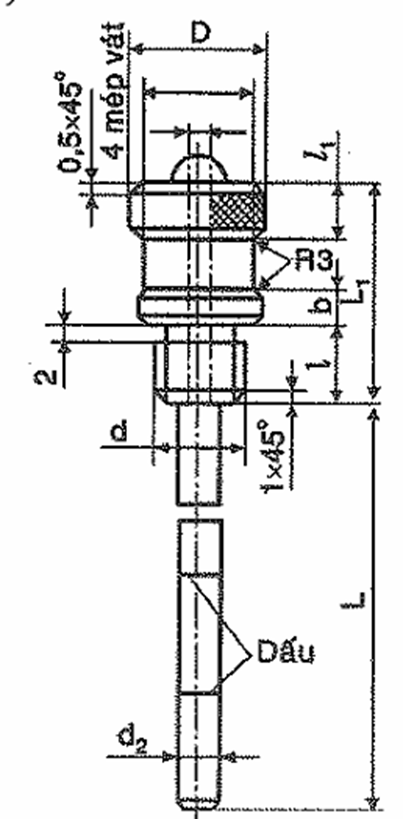
\includegraphics[width=0.5\textwidth]{pictures/quethamdau.png}
    \caption{Que thăm dầu}
\end{figure}
\cleardoublepage
\subsection{Nút tháo dầu}
Chọn nút tháo dầu dạng vít ren trụ tròn M20x1.5 với thông số như sau:
\begin{table}[H]
    \centering
    \begin{tabular}{|c|c|c|c|c|c|c|c|c|c|c|}
    \hline
    $\mathbf{d1}$ & $\mathbf{D}$ & $\mathbf{D1}$ & $\mathbf{L}$ & $\mathbf{l}$ & $\mathbf{b}$ & $\mathbf{s}$ & $\mathbf{t}$ & $\mathbf{d2}$ & $\mathbf{D2}$ & $\mathbf{D2}$ \\
    \hline
    M20x1.5 & 30 & 25.4 & 30 & 15 & 4 & 22 & 2.5 & 20 & 32 & 3 \\
    \hline
    \end{tabular}
    \caption{Thông số nút tháo dầu}
\end{table}
\begin{figure}[H]
    \centering
    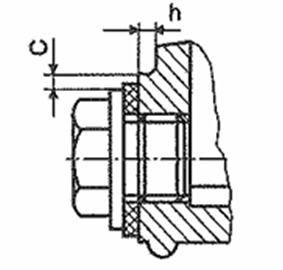
\includegraphics[width=0.5\textwidth]{pictures/nut.png}
    \caption{Nút tháo dầu}
\end{figure}

\subsection{Cửa thăm và nút thông hơi}
Chọn nắp cửa thăm và nút thông hơi có kích thước như sau:
\begin{table}[H]
    \centering
\begin{tabular}{|c|c|c|c|c|c|c|c|c|}
\hline
A & B & A1 & B1 & C & K & R & Dimension & Quantity \\
\hline
40 & 40 & 80 & 90 & 65 & 30 & 10 & M8 & 4 \\
\hline
\end{tabular}
\caption{Thông số cửa thăm và nút thông hơi}
\end{table}
\begin{figure}[H]
    \centering
    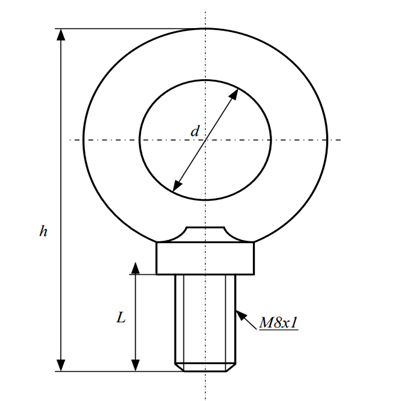
\includegraphics[width=0.5\textwidth]{pictures/vitvong.png}
    \caption{Cửa thăm và nút thông hơi}
\end{figure}
\subsection{Vòng chắn dầu}
Gồm 3 rãnh tiết diện tam giác đều có góc ở đỉnh là 60 độ, khoảng cách giữa các đỉnh là 3mm. Mép ngoài của vòng cách thành trong của hộp một khoảng bằng 3mm. 
\begin{figure}[H]
    \centering
    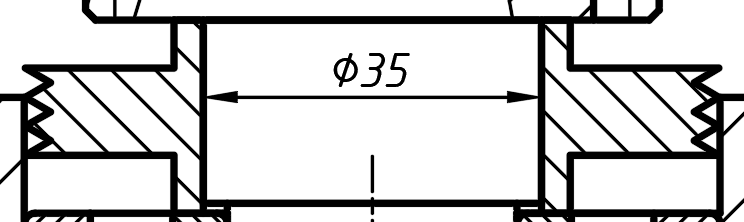
\includegraphics[width=0.5\textwidth]{pictures/vongchandau.png}
    \caption{Vòng chắn dầu}
\end{figure}
\subsection{Chốt định vị}
Dùng để xác định vị trí làm việc êm của hộp giảm tốc sau khi lắp ráp, hình dạng và kích thước được cho bởi:
\begin{figure}[H]
    \centering
    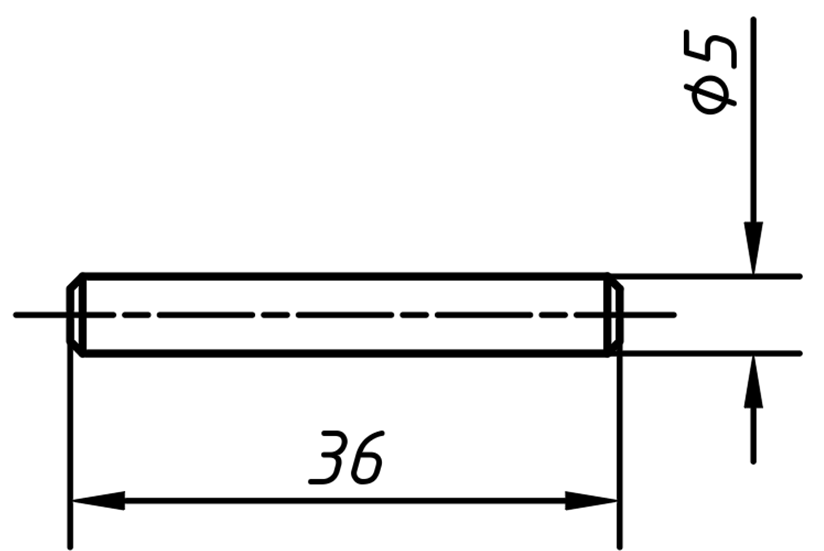
\includegraphics[width=0.5\textwidth]{pictures/chotdinhvi.png}
    \caption{Chốt định vị}
\end{figure}
\subsection{Vòng phớt}
Vòng phớt là loại lót kín động gián tiếp nhằm mục đích bảo vệ ổ khỏi bụi bặm, chất bẩn, hạt cứng và các tạp chất khác xâm nhập vào ổ. Những chất này làm ổ chóng bị mài mòn và bị han gỉ. Ngoài ra, vòng phớt còn đề phòng dầu chảy ra ngoài. Tuổi thọ ổ lăn phụ thuộc rất nhiều vào vòng phớt. Vòng phớt được dùng khá rộng rãi do có kết cấu đơn giản, thay thế dễ dàng. Tuy nhiên có nhược điểm là chóng mòn và ma sát lớn khi bề mặt trục có độ nhám cao.\\
Theo tiêu chuẩn, chọn vòng phớt có đường kính trong là 25mm cho trục dẫn và vòng phớt có đường kính trong là 38mm cho trục bị dẫn. Các kích thước khác của vòng phớt được lấy theo tiêu chuẩn.
\begin{figure}[H]
    \centering
    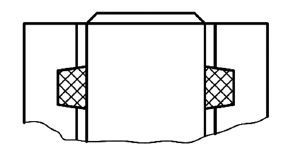
\includegraphics[width=0.5\textwidth]{pictures/vongphot.png}
    \caption{Vòng phớt}
\end{figure}
\cleardoublepage
    \chapter{Dung sai và lắp ghép}
Căn cứ vào các yêu cầu làm việc của từng chi tiết trong hộp giảm tốc, ta chọn các
kiểu lắp ghép sau:
\section{Dung sai ổ lăn}
Vòng trong ổ lăn chịu tải tuần hoàn, ta lắp ghép theo hệ thống trục lắp trung gian để
vòng ổ không trượt trên bề mặt trục khi làm việc. Do đó, ta phải chọn mối lắp k6, lắp
trung gian có độ dôi, tạo điều kiện mòn đều ổ (trong quá trình làm việc nó sẽ quay làm
mòn đều).
Vòng ngoài của ổ lăn không quay nên chịu tải cục bộ, ta lắp theo hệ thống lỗ. Để ổ có
thể di chuển dọc trục khi nhiệt đô tăng trong quá trình làm việc, ta chọn kiểu lắp trung
gian H7.
\section{Lắp ghép bánh răng trên trục}
Bánh răng lắp lên trục chịu tải vừa, tải trọng tĩnh, va đập nhẹ, ta chọn kiểu lắp ghép
H7/k6.
\section{Lắp ghép vòng chắn dầu trên trục}
Để dễ dàng cho tháo lắp, ta chọn kiểu lắp trung gian H8/Js7
\section{Lắp ghép then}
Theo chiều rộng, chọn kiểu lắp trên trục và kiểu lắp trên bạc là Js9/h9.
Theo chiều cao, sai lệch giới hạn kích thước then là h11.
Theo chiều dài, sai lệch giới hạn kích thước then là h14.
\cleardoublepage
\textbf{Bảng dung sai lắp ráp}
\begin{table}[H]
    \centering
    \begin{tabular}{|c|p{4cm}|>{\centering\arraybackslash}p{2cm}|>{\centering\arraybackslash}m{3cm}|>{\centering\arraybackslash}m{3cm}|}
    \hline
    \textbf{Trục} & \textbf{Mối ghép} & \textbf{Kiếu lắp} & \textbf{Sai lệch giới hạn của lỗ, $\mu$m} & \textbf{Sai lệch giới hạn của trục, $\mu$m} \\
    \hline
    \multirow{5}{*}{\textbf{I}}& Vòng ngoài ổ lăn & H7 & 0...+30 & \\
    \cline{2-5}
    & Vòng trong ổ lăn & k6 & & +2...+15 \\
    \cline{2-5}
    & Vòng chắn dầu & H8/js7 & 0...+39 & -12...+12 \\
    \cline{2-5}
    & Nắp ổ lăn trục I với vỏ hộp & H7/e8 & 0...+30 & -106...-60 \\
    \hline
    \multirow{6}{*}{\textbf{II}} & Nối trục đàn hồi & H7/k6 & 0...+16 & +2...+18 \\
    \cline{2-5}
    & Bánh răng bị dẫn & H7/k6 & 0...+25 & +2...+18 \\
    \cline{2-5}
    & Vòng ngoài ổ lăn & H7 & 0...+30 & \\
    \cline{2-5}
    & Vòng trong ổ lăn & k6 & & +2...+18 \\
    \cline{2-5}
    & Vòng chắn dầu & H8/js7 & 0...+39 & -12...+12 \\
    \cline{2-5}
    & Nắp ổ lăn trục II với vỏ hộp & H7/e8 & 0...+30 & -126...-72 \\
    \hline
    \end{tabular}
\end{table}

    \chapter{Thiết kế hệ thống truyền động}
\section{Tính bộ phận công tác}
\subsection{Tính bước của trục vít tải}
\begin{itemize}
    \item Ta chọn vật liệu là Inox 304 vì nó có độ bền cao, khả năng chống ăn mòn tốt phù hợp với môi trường làm việc của máy ép bùn.
    \item Ta sử dụng vít tải quay chậm để vận chuyển vật liệu theo phương nằm ngang. 
    \item Khi trục vít quay thì vật liệu được nâng lên và cả khối vật liệu bị nghiêng đi một góc $\varphi $ như hình dưới, tại đó trọng lượng của vật liệu sẽ cân bằng với lực ma sát của vật liệu với thành máy.
\end{itemize}
\begin{figure}[H]
    \centering
    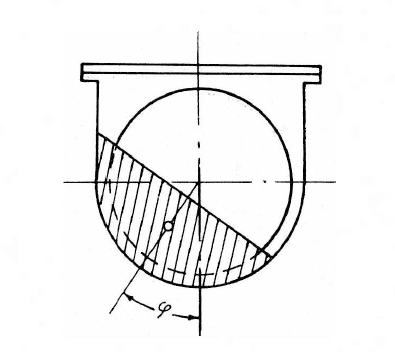
\includegraphics[width=0.5\textwidth]{pictures/vittai1.png}
    \caption{Sự phân bố của vật liệu khi trục vít tải quay}
\end{figure}

\begin{itemize}
    \item Bước của trục vít (hay khoảng cách giữa các cánh vít) đối với vật liệu dạng bột hoặc hạt nhỏ được xác định là:
    \[
        S = (0.7 \div 1)D = 1 \cdot 225 = 225 (mm) 
    \]
\end{itemize}

\subsection{Diện tích tiết diện ngang do vật liệu chiếm trong thành máy}
\[
    F = \frac{\pi\cdot D^2}{4}\mu \cdot K = \frac{\pi\cdot 0.225^2}{4}\cdot 0.35\cdot 1 = 0.0139 (m^2)
\]
Trong đó: 
\begin{itemize}
    \item D = 225 mm, là đường kính của vít tải
    \item $\mu$ là hệ số chứa vật liệu trong thành máy. Với vật liệu dạng bột ta chọn $\mu = 0.35$
    \item K là hệ số chỉ sự giảm tiết diện do góc nghiêng đặt vít tải. Với góc nghiêng bằng $0^{\circ}$ ta chọn $K = 1$
\end{itemize}
\subsection{Vận tốc chuyển vật liệu dọc theo trục vít}
\[
    v = \frac{S\cdot n_{ct}}{60} = \frac{0.225\cdot 118.85}{60} = 0.4434 (m/s)
\]
Trong đó: 
\begin{itemize}
    \item $S = 225 mm$: bước của vít tải
    \item $n_{ct} = 118.85$ vòng/phút: số vòng quay của trục vít tải
\end{itemize}
\subsection{Xác định năng xuất máy}
\[
    Q = 3600F\cdot v\cdot \rho = 3600\cdot 0.0139\cdot 0.4434\cdot 1000 = 22187.74 (kg/h)
\]
Trong đó:
\begin{itemize}
    \item $F = 13916.27 mm^2$: diện tích ngang do vật liệu chiếm trong thành máy
    \item $v = 0.4434$ m/s: vận tốc chuyển vật liệu dọc theo trục vít
    \item $\rho = 1000$ kg/m$^3$: khối lượng riêng của bùn
\end{itemize}
\section{Thùng cấp liệu}
\begin{itemize}
    \item Vật liệu: Inox 304
    \item Kích thước: 170x170x75 mm
    \item Tùy theo như cầu sử dụng mà có thể thay đổi kích thước của thùng cấp liệu cho phù hợp với yêu cầu của máy.
\end{itemize}
\begin{figure}[H]
    \centering
    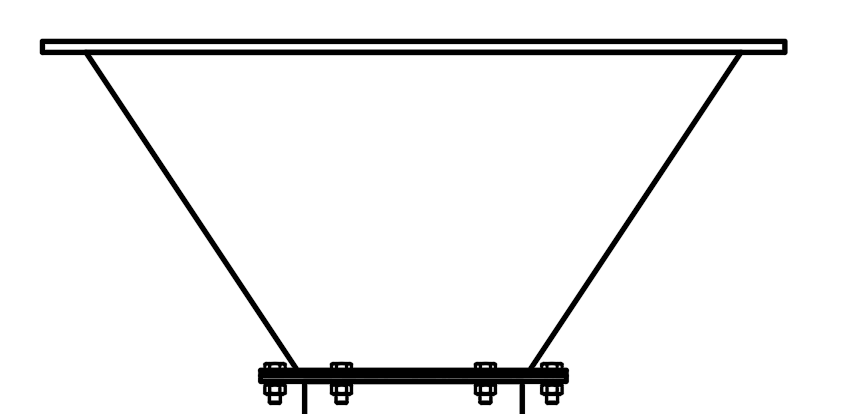
\includegraphics[width=0.5\textwidth]{pictures/thungcap.png}
    \caption{Thùng cấp liệu}
\end{figure}

\section{Vít tải}
\begin{itemize}
    \item Vật liệu: Inox 304
    \item Đường kính: 225 mm
    \item Tùy theo như cầu sử dụng mà có thể thay đổi kích thước của vít tải cho phù hợp với yêu cầu của máy.
\end{itemize}
\begin{figure}[H]
    \centering
    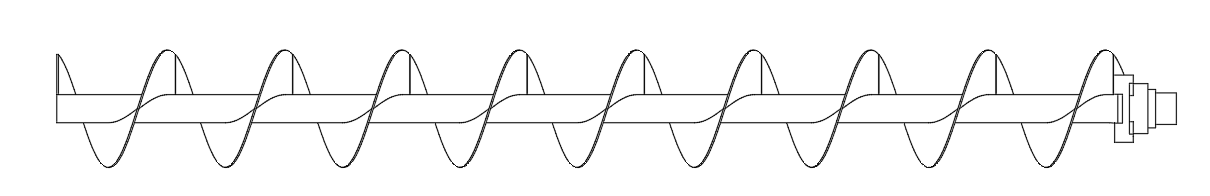
\includegraphics[width=1\textwidth]{pictures/vit.png}
    \caption{Vít tải}
\end{figure}

\section{Thân máy hình máng}
\begin{itemize}
    \item Vật liệu: Inox 304
    \item Đường kính: 300 mm
    \item Thân máy được nối với thùng cấp liệu bằng bulong và đai ốc.
    \item Thân máy có chỗ xả liệu để xả bùn ra ngoài.
\end{itemize}
\begin{figure}[H]
    \centering
    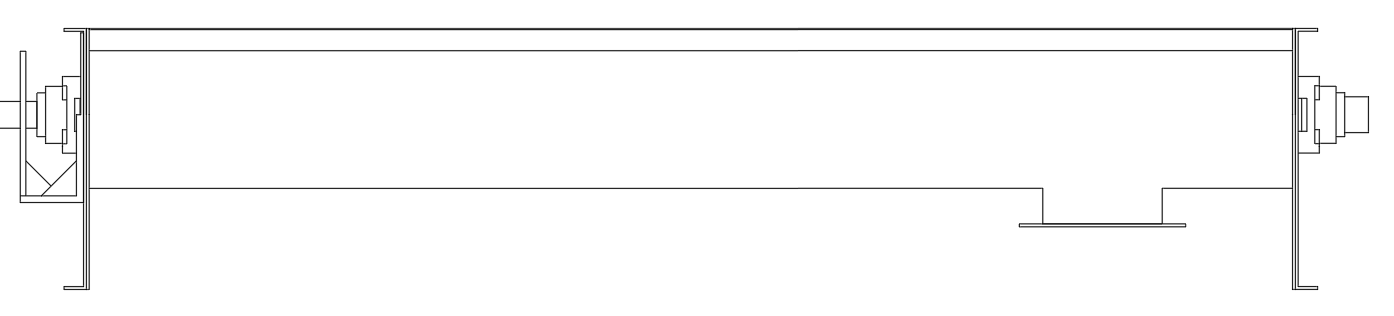
\includegraphics[width=1\textwidth]{pictures/than.png}
    \caption{Thân máy hình máng}
\end{figure}

\section{Bệ đỡ động cơ và hộp giảm tốc}
\begin{itemize}
    \item Vật liệu: Thép.
    \item Cố định các đơn vị lắp lên bệ đỡ bằng bulong và đai ốc.
    \item Có thể sử dụng phương pháp hàn để cố định các bệ đỡ.
\end{itemize}
\begin{figure}[H]
    \centering
    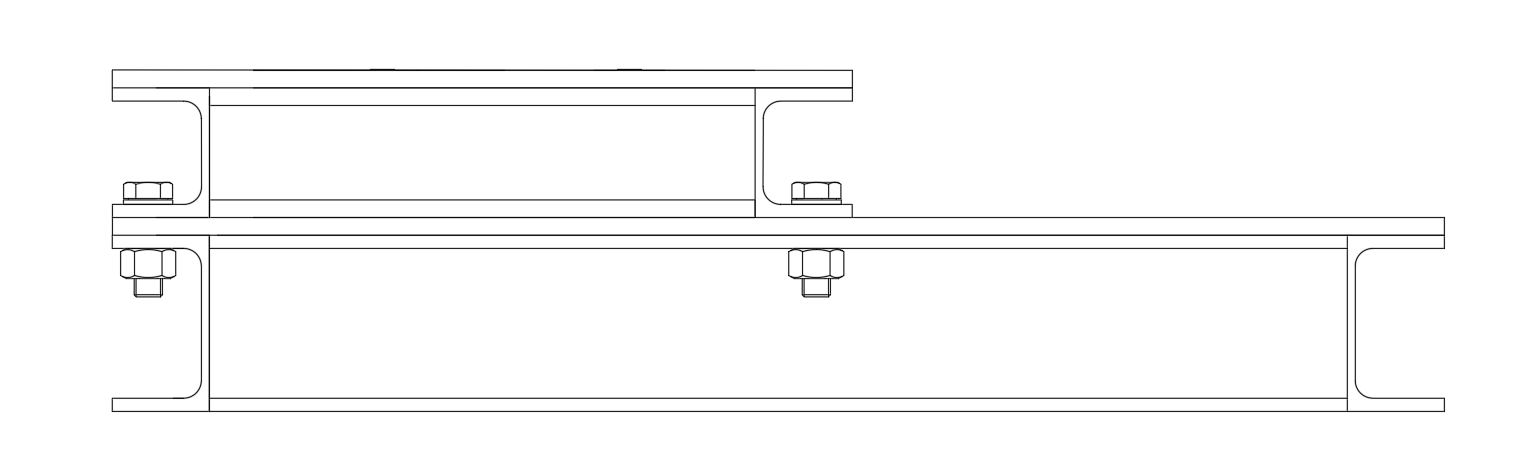
\includegraphics[width=1\textwidth]{pictures/be.png}
    \caption{Bệ đỡ động cơ và hộp giảm tốc}
\end{figure}

\section{Bộ phận căng đai}
\begin{itemize}
    \item Chế tạo từ các tấm thép khi sản xuất đơn chiếc.
    \item Sử dụng gang xám khi sản xuất hàng loạt.
    \item Bộ phận căng đai được lắp trên bệ đỡ động cơ và hộp giảm tốc.
    \item Căng đai bằng phương pháp dịch chuyển động cơ tịnh tiến.
    \item Cố định với bệ đỡ và động cơ bằng bulong và đai ốc.
\end{itemize}
\begin{figure}[H]
    \centering
    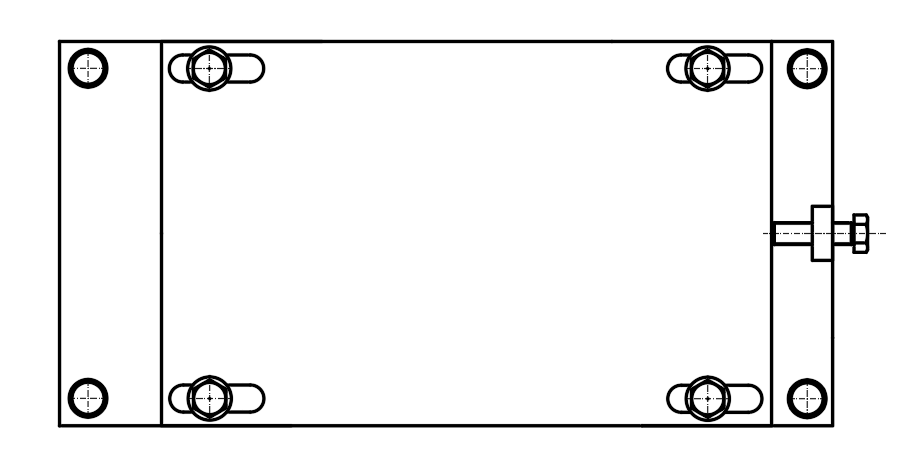
\includegraphics[width=0.7\textwidth]{pictures/cangdai.png}
    \caption{Bộ phận căng đai}
\end{figure}

\section{Gối đỡ vòng bi}
\begin{itemize}
    \item Mã sản phẩm: FY 45 FM
    \item Nhà sản xuất: SKF
    \item Đường kính trục: 45 mm
    \item Kiểu gối đỡ: Mặt bích vuông 4 lỗ
    \item Vật liệu vỏ: Gang đúc
    \item Loại vòng bi: Vòng bi cầu (ball bearing)
    \item Tải trọng động: 33,2 kN
    \item Tải trọng tĩnh: 21,6 kN
    \item Tốc độ tối đa: 4.300 vòng/phút
\end{itemize}
\begin{figure}[H]
    \centering
    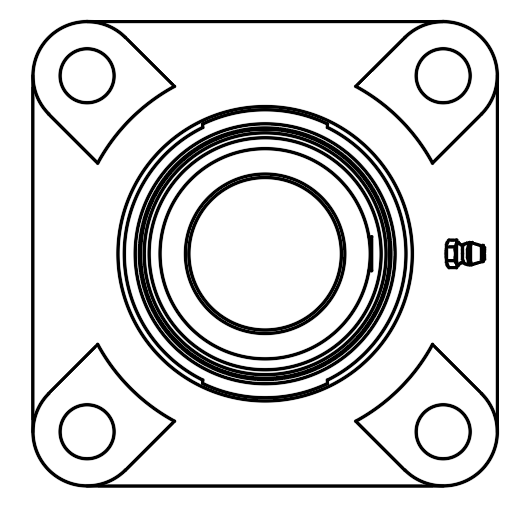
\includegraphics[width=0.4\textwidth]{pictures/goi.png}
    \caption{Gối đỡ vòng bi}
\end{figure}
    
    \begin{thebibliography}{9}
        \bibitem{key1}
        Nguyễn Hữu Lộc, Cơ sở thiết kế máy. Nhà xuất bản Đại học quốc gia TP. Hồ Chí Minh, 2013.
        \bibitem{key2}
        Trịnh Chất – Lê Văn Uyển, Tính toán thiết kế hệ dẫn động cơ khí, tập 1, Nhà xuất bản giáo dục, 2006.
        \bibitem{key3}
        Trịnh Chất – Lê Văn Uyển, Tính toán thiết kế hệ dẫn động cơ khí tập 2, Nhà xuất bản giáo dục, 2006.
        \bibitem{key4}
        Nguyễn Hữu Lộc, Thiết kế máy - chi tiết máy, Nhà xuất bản Đại học quốc gia TP. Hồ Chí Minh, 2020.
        \bibitem{key5}
        Hồ Lệ Viên, Các máy gia công vật liệu rắn và dẻo, Nhà xuất bản khoa học và kỹ thuật 
        \end{thebibliography}
\end{document}